\documentclass[12pt]{article}
\usepackage{algorithm}
\usepackage{algpseudocode}
\usepackage{amsmath}
\usepackage{amssymb}
\usepackage{amsthm}
\usepackage[titletoc]{appendix}
\usepackage{array}
\usepackage[english]{babel}
\usepackage{booktabs}
\usepackage{cancel}
\usepackage{chngcntr}
\usepackage{color}
\usepackage{eqparbox}
\usepackage{float}
\usepackage[margin=1in]{geometry}
\usepackage{graphicx}
\usepackage[colorlinks=true]{hyperref}
% *must* be loaded after hyperref
\usepackage[toc, acronym, numberedsection=nameref]{glossaries}
\usepackage[utf8]{inputenc}
\usepackage{lipsum}
\usepackage{mathtools}
\usepackage[cache=false]{minted}
\usepackage{parskip}
\usepackage{pgfplots}
\usepackage{scalerel}
\usepackage{skull}
\usepackage{subcaption}
\usepackage{titling}
\usepackage{textcomp}
\usepackage{tikz}
\usepackage[compact, explicit]{titlesec}
\usepackage{textcomp}
\usepackage[nottoc]{tocbibind}
\usepackage[textsize=small]{todonotes}
\usepackage[normalem]{ulem}

% Document Settings

\definecolor{__minted_background_color}{rgb}{0.95, 0.95, 0.98}
\definecolor{__minted_highlight_color}{rgb}{0.88, 0.88, 1.0}
\setminted{autogobble=true,
    style=tango,
    breaklines,
    bgcolor=__minted_background_color,
    highlightcolor=__minted_highlight_color,
    mathescape, % Escape math mode everywhere.
    texcomments,  % Enable latex code inside of comments. Useful for referencing equations.
}

\usetikzlibrary{arrows, backgrounds, lindenmayersystems, matrix, positioning, shapes}
\pgfplotsset{compat=1.15}
\numberwithin{algorithm}{section}
\numberwithin{equation}{section}
\numberwithin{figure}{section}
% \numberwithin{section}{part}
\counterwithin*{section}{part}

% Sets the width of the margin TODO notes
\setlength{\marginparwidth}{0.84in}
\reversemarginpar{}

% hex #184c9a
\definecolor{__glossary_entry_color}{rgb}{0.094, 0.298, 0.604}
\renewcommand{\glstextformat}[1]{\textbf{\textcolor{__glossary_entry_color}{#1}}}

% Add glos: to the beginning of the glossary labels.
\renewcommand*{\glsautoprefix}{glos:}

% All I want is to have comment italicized, but I cant figure out how
% to properly modify the existing \Comment macro.
% \algrenewcomment[1]{\hfill\eqparbox{COMMENT}{\textit{// #1}}}
\algnewcommand{\IComment}[1]{\Comment{\textit{#1}}}
% enable \autoref with algorithms
\newcommand{\algorithmautorefname}{Algorithm}

% TODO: Should this path be relative to the document root or this file?
\graphicspath{{./figures/}}

% Document Definitions

\newcommand{\C}{\mathbb{C}}
\newcommand{\R}{\mathbb{R}}
\newcommand{\Z}{\mathbb{Z}}
\newcommand{\N}{\mathbb{N}}
\renewcommand{\O}{\mathcal{O}}

\theoremstyle{definition}
\newtheorem{defn}{Definition}[section]

\theoremstyle{plain}
\newtheorem{thm}{Theorem}[section]

\renewcommand{\qedsymbol}{$\skull$}

% An inline TODO command. Doesn't play nicely with \todotableofcontents
\newcommand\todoinline[2][]{\todo[inline, caption={TODO}, #1]{
        \begin{minipage}{\textwidth-4pt}#2\end{minipage}}}

% Draw clouds around things. Useful in mathematical proofs.
\newcommand{\cloud}[4][\dots]{%
    \raisebox{-0.4\height}{%
        \begin{tikzpicture}
            \node [cloud,
                draw,
                cloud puffs=#2,
                cloud ignores aspect,
                minimum height=#3,
                minimum width=#4] {#1};
        \end{tikzpicture}
    }
}

% % make each \section a problem.
% \titleformat{\section}[runin]{\large\bfseries}{}{0pt}{\titlerule[1.5pt]\newline\vspace*{-4pt}
%     Problem\quad\thesection\newline}[\vspace{0.01ex}{\titlerule[1.5pt]}]

% Make autorefs to sections say "Problem x"
% \AtBeginDocument{%
% \renewcommand{\sectionautorefname}{Problem}
% }

% Use \ceil*{} or \floor*{}
\DeclarePairedDelimiter{\ceil}{\lceil}{\rceil}
\DeclarePairedDelimiter{\floor}{\lfloor}{\rfloor}


\title{Homework 4}
\author{Austin Gill \\ Kyle MacMillan}
\date{April 26, 2019}

\begin{document}
\maketitle
\begingroup
\hypersetup{linkcolor=black}
\tableofcontents
\endgroup

The code for this homework assignment can be found at \url{https://github.com/macattackftw/fractal_trees}.
The README explains how to use the scripts for each problem.

A considerable amount of implementation details, and the reasoning behind certain unsettling decisions, have been left out.
Of notable interest is how to install the prerequisite software, including Blender and the appropriate Python packages.
Feel free to contact the authors at \href{mailto:austin.gill@mines.sdsmt.edu}{austin.gill@mines.sdsmt.edu} and \href{mailto:kyle.macmillan@mines.sdsmt.edu}{kyle.macmillan@mines.sdsmt.edu} for more details.

Also note that there are a great many links to some of our results that are not possible to embed in a PDF document.
Particularly, interactive 3D renderings of many of the fractals are hosted online.

\newpage

\part{Fractals}
\vspace{2in}
\begin{figure}[H]
    \centering
    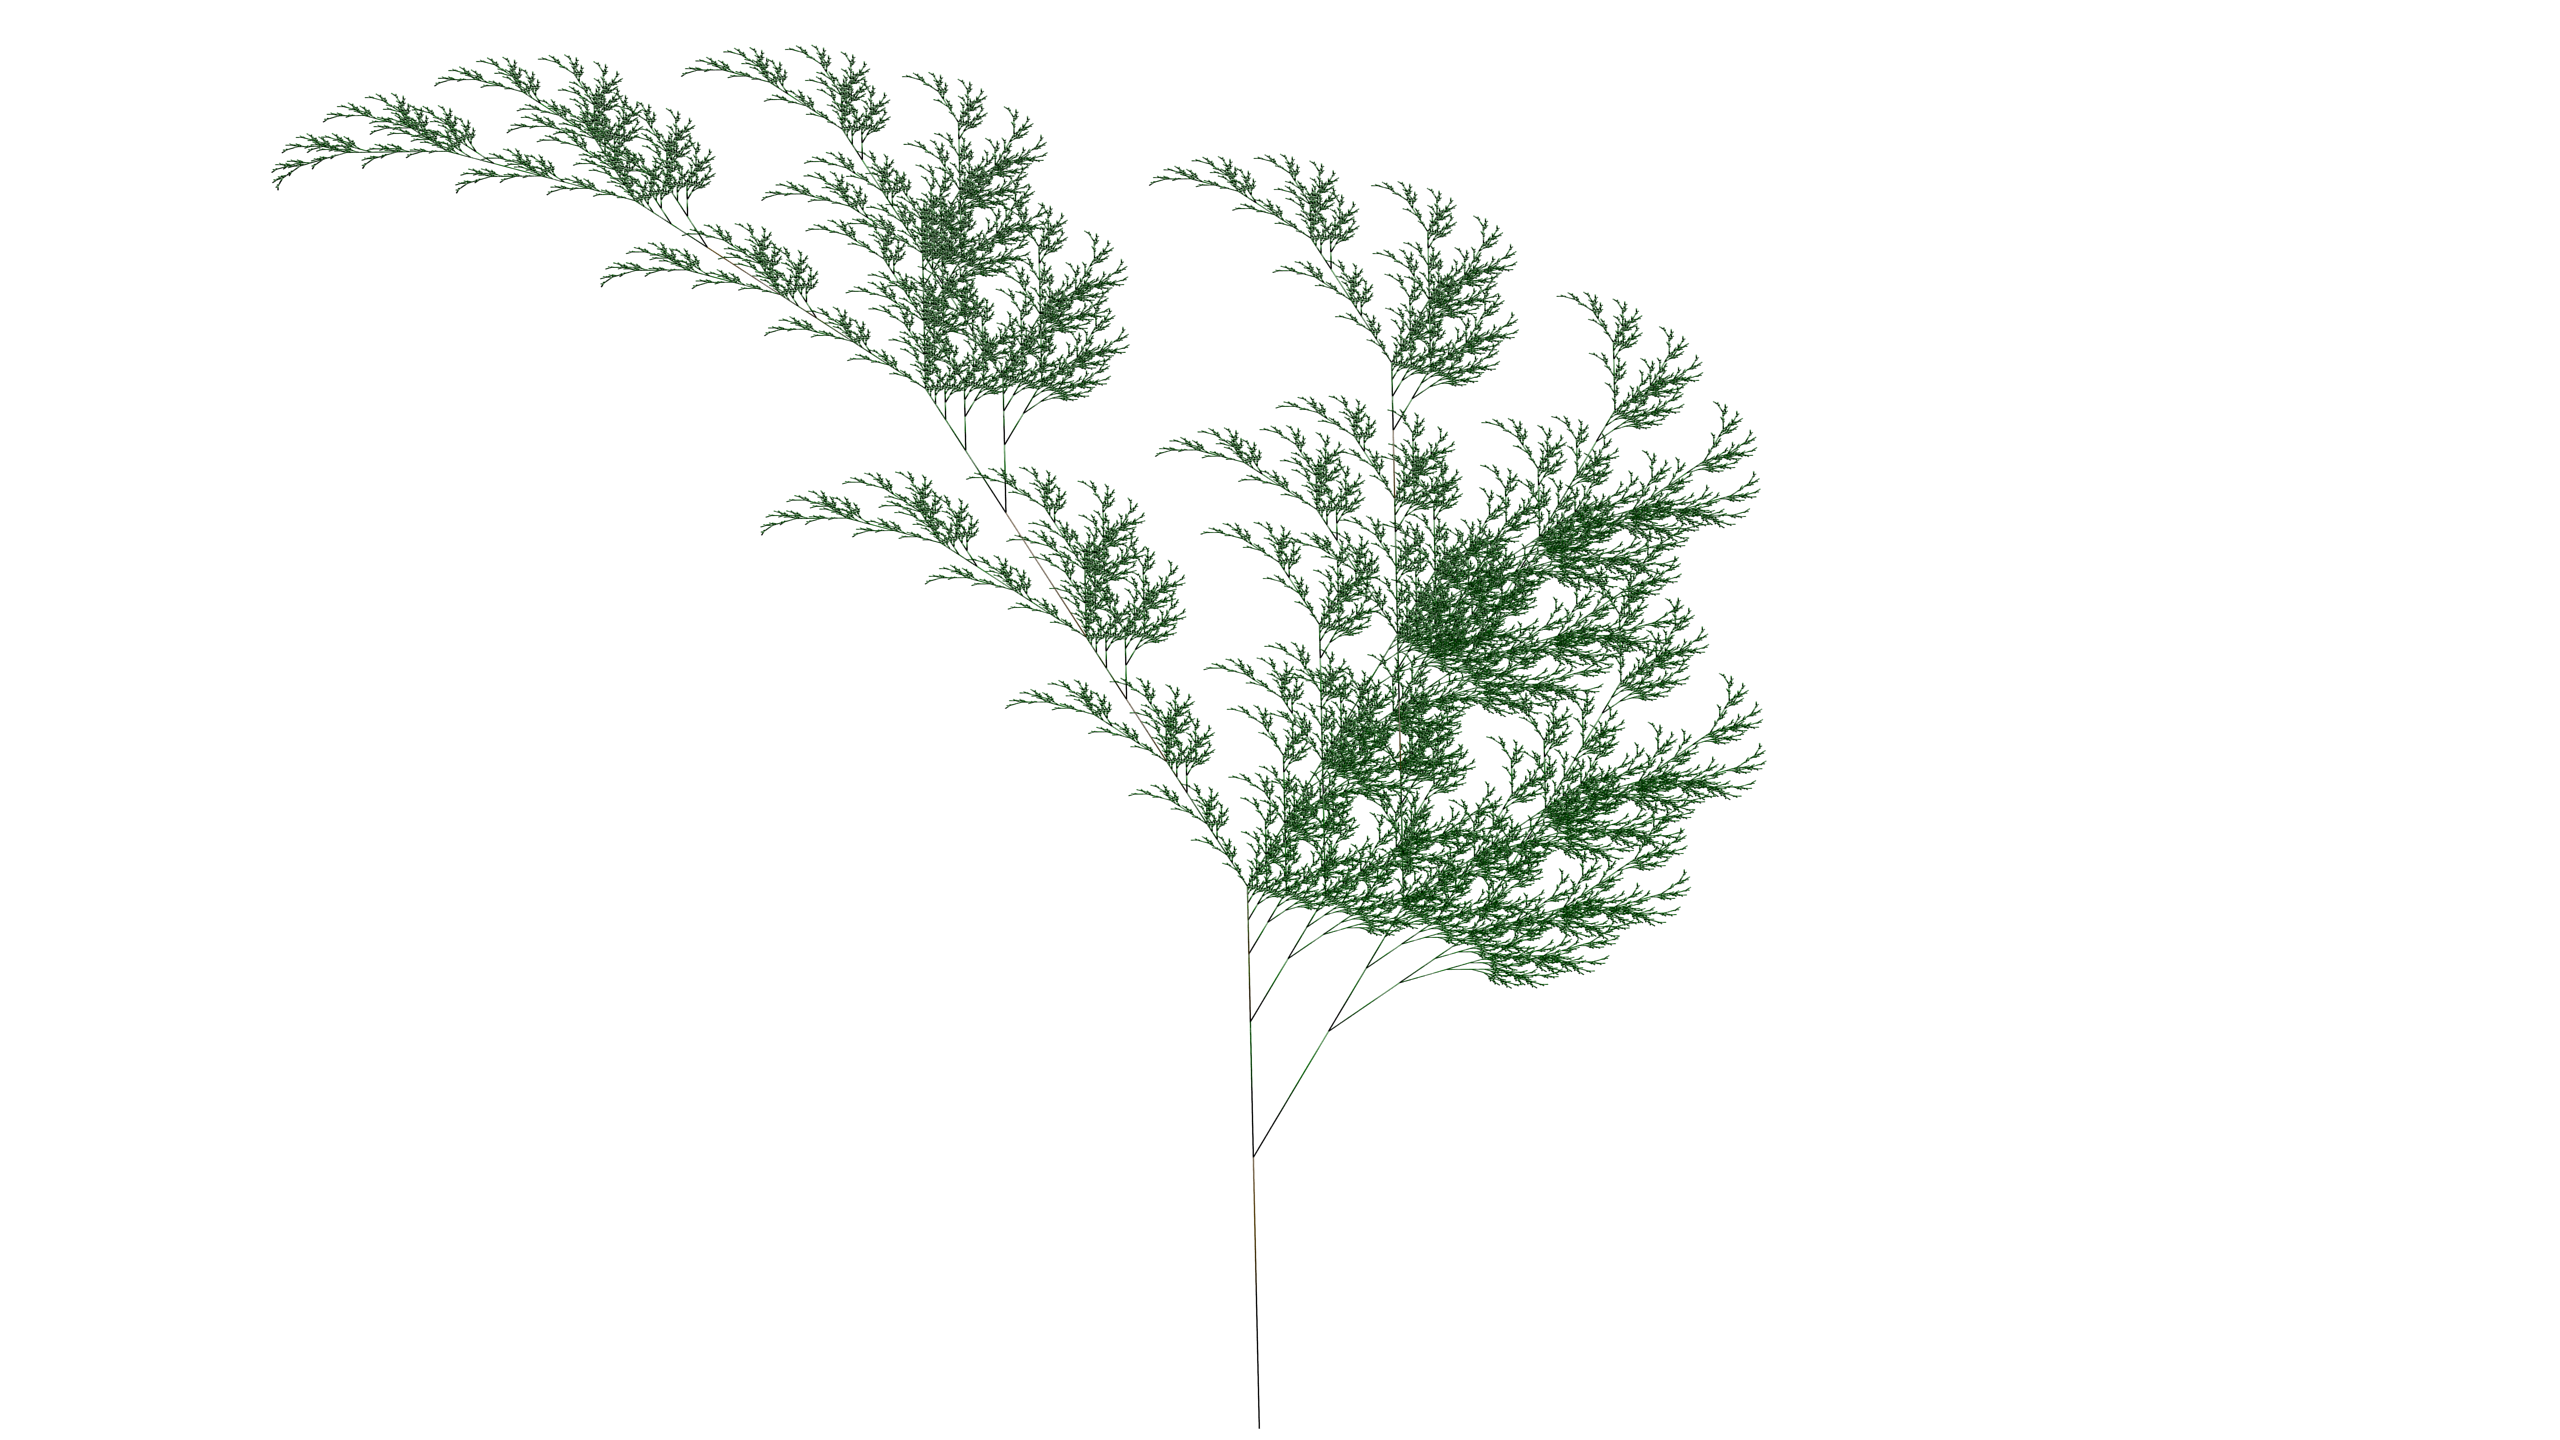
\includegraphics[width=\textwidth]{figures/L-systems/a.png}
\end{figure}
% !TeX root = ../hw4.tex
\section{Generating a Simple Fractal Tree}

\subsection{Statement}

Generate a fractal tree by repeating a ``fork'' shape with default angle of $45^\circ$.
Scale each repetition of the whole fractal by $\frac{1}{3}$ each iteration.

Experiment with different angles.

\subsection{Method}\label{sec:l-system-method}

\subsubsection{Lindenmayer Systems}
Lindenmayer Systems are commonly referred to as
\href{https://en.wikipedia.org/wiki/L-system}{L-Systems}. An L-System takes a
series of production rules and applies them to an
\href{https://en.wikipedia.org/wiki/Axiom}{axiom}, or initial string for a
defined number of iterations. To define these L-Systems our approach utilizes a
JSON configuration file to store the system's variables:

\begin{minted}{json}
{
    "unit": 1,
    "angle": 0.392699082,
    "radius": null,
    "proportion": null,
    "axiom": "G",
    "iterations": 6,
    "randomness": null,
    "rules": {
        "G": "F+[[G]-G]-F[-FG]+G",
        "F": "FF"
    }
}
\end{minted}

A description for each of the JSON parameters is given in \autoref{tab:json_format}.

\begin{table}[H]
    \centering
    \caption{JSON config file parameters}\label{tab:json_format}
    \begin{tabular}{@{}cl@{}}
        \toprule
        \textbf{Name} & \textbf{Description}                                 \\ \midrule
        unit          & Length of a segment                                  \\
        angle         & Angle (radians) applied to \mintinline{text}{+-^v<>} \\
        radius        & Radius for segments                                  \\
        proportion    & Changes radius to a proportion of length             \\
        axiom         & Initial string                                       \\
        iterations    & Number of times to iterate                           \\
        randomness    & Perturbation applied to angle                        \\
        rules         & Denotes what becomes of characters                   \\ \bottomrule
    \end{tabular}
\end{table}

% \todoinline[caption=Define an L-System]{Define an L-System, production rules, and specify the meaning of the different commands.}

\subsubsection{The Lindenmayer System for the Given Problem}
The problem required us to ``shrink'' the original to 1/3 size and apply it to
each angled protrusion. We accomplished that by coming up with an L-System
that grew each previous iteration by a factor of 3 each time it went through a
new iteration. This system is given in \autoref{code:prob1_json}.

\begin{listing}[H]
    \begin{minted}{json}
        {
            "unit": 1,
            "angle": 0.785398163,
            "radius": null,
            "proportion": null,
            "axiom": "F",
            "iterations": 7,
            "randomness": null,
            "rules": {
                "F": "GGG[-F][F][+F]",
                "G": "GG"
            }
        }
    \end{minted}
    \caption{The JSON configuration for the given problem}\label{code:prob1_json}
\end{listing}

We were tasked with changing the angle to 90° which resulted in a
Christmas tree-like structure. We were also tasked with changing the angle to
120° and it resulted in something similar to a
\href{https://en.wikipedia.org/wiki/Sierpi\%C5\%84ski\_triangle}{Sierpiński triangle}.
All three versions are viewable via
\href{https://sketchfab.com/macattackftw/collections/problem-1}{Sketchfab}.

\begin{itemize}
    \item \href{https://sketchfab.com/3d-models/prob1-45-a97f7475b6964b9c930796ba985ac255}{45 degrees}
    \item \href{https://sketchfab.com/3d-models/8c7a25615cee4fb4a51ab3deeae154a0}{90 degrees}
    \item \href{https://sketchfab.com/3d-models/b36c6e912ee548b9a549bd8e0bb273c8}{120 degrees}
\end{itemize}

% \todoinline[caption=Give l-system for given problem]{Give the L-System for given problem and discuss how it might be improved or modified.}

\subsubsection{Extending the Lindenmayer Systems to 3D}
The book mentioned symbols to expand the generation into different dimensions.
We borrowed some of those symbols to generate L-Systems that expanded in the
$x$, $y$, and $z$ dimensions. We applied this
concept to the 45° version of problem 1 and it resulted in a very
\href{https://sketchfab.com/3d-models/prob1-3d-236e501897a945d0a3eb5e4cba37fa3a}{symmetrical tree}.
The JSON configuration for the given 3D rendering is shown in \autoref{code:prob1_3D_json}.

\begin{listing}[H]
    \begin{minted}{json}
        {
            "unit": 1,
            "angle": 0.785398163,
            "radius": null,
            "proportion": null,
            "axiom": "F",
            "iterations": 3,
            "randomness": null,
            "rules": {
                "F": "GGG[-F][F][+F][vF][^F][<F][>F]",
                "G": "GG"
            }
        }
    \end{minted}
    \caption{Problem 1 3D JSON}\label{code:prob1_3D_json}
\end{listing}

Transitioning to 3D space was incredibly simple due to Blender's mathutils
Matrix module as seen in the
\autoref{code:roll_pitch_yaw}. We spent a lot of
time attempting to manipulate Quaternions but found the mathutils module met
all of our requirements and didn't give us a headache.

\begin{listing}[H]
    \begin{minted}{python}
        def yaw(self, angle):
            """Yaw the Turtle around its local Z axis."""
            self.mat = matmul(self.mat, Matrix.Rotation(angle, 4, "Z"))

        def pitch(self, angle):
            """Pitch the Turtle around its local Y axis."""
            self.mat = matmul(self.mat, Matrix.Rotation(angle, 4, "Y"))

        def roll(self, angle):
            """Roll the Turtle around its local X axis."""
            self.mat = matmul(self.mat, Matrix.Rotation(angle, 4, "X"))
    \end{minted}
    \caption{Roll, Pitch, Yaw code}\label{code:roll_pitch_yaw}
\end{listing}

Angle commands such as \mintinline{text}{^} were mapped to pitch function described in
the \autoref{code:roll_pitch_yaw}. So the turtle
would pitch $\theta$ and if the angle command was \mintinline{text}{v} it would pitch
$-\theta$.

% \todoinline[caption=Defined new 3D commands]{
%     Show how to add more commands to extend the L-Systems into 3D.

%     Mention that we implemented this as the book suggested --- by creating a 3D turtle that can yaw, pitch, and roll.

%     Give minimal examples of each command.
% }

\subsubsection{Further Extensions of the Lindenmayer Systems}
Another concept the book mentioned was moving forward without drawing a line.
This was accomplished with symbols \mintinline{text}{f} and \mintinline{text}{g}. Utilizing this
concept we were able to reproduce the
\href{https://sketchfab.com/3d-models/cantor-f645d6ae69a748a283a737f44660c5f6}{Cantor Set}.

We were making plant-like structures so we decided that anything over length 1
would be a ``branch'' and anything else was a ``leaf''. This led to much more
plant-like visualization of the L-Systems. A good example of this can be seen
in \autoref{fig:a_3d} and \autoref{fig:prob1_3d}. We did not have to stop
at 2 colors. We could have added any number of colors and based it on the
length or on the iteration. We chose 2 because it demonstrated the concept and
made the resulting system look better.

\begin{figure}[H]
    \centering
    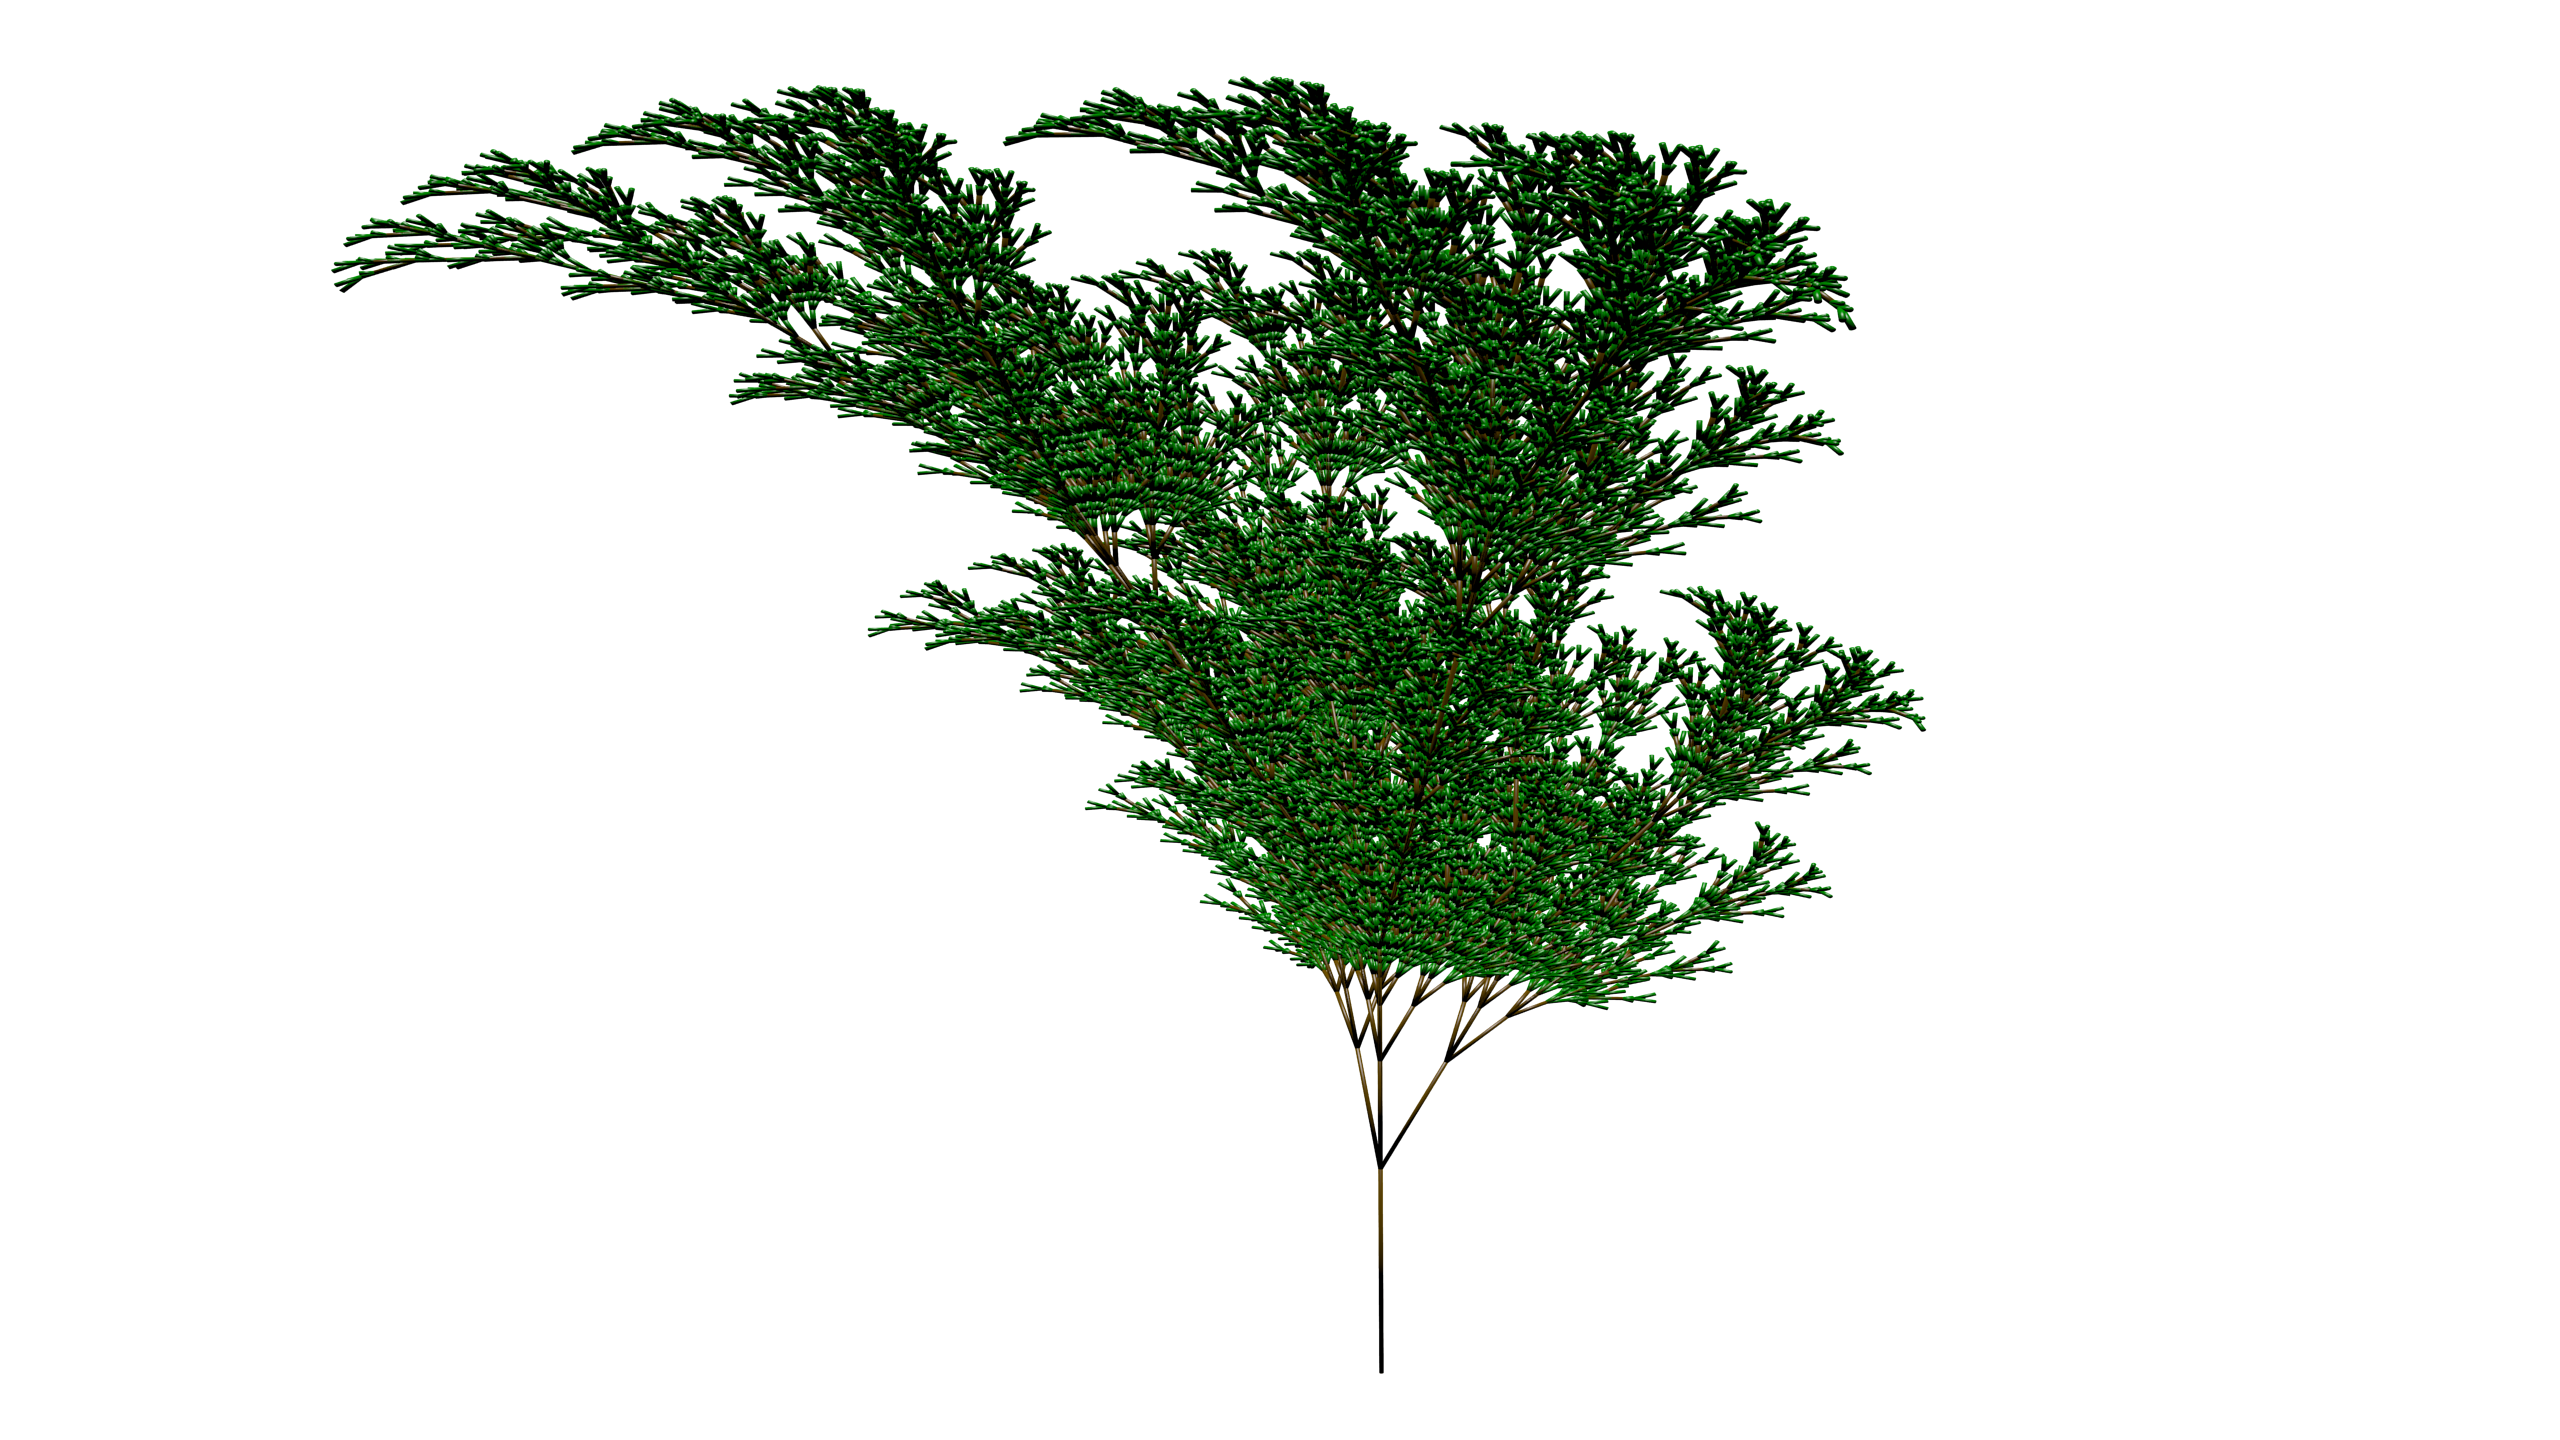
\includegraphics[width=0.75\textwidth]{figures/L-systems/a3d.png}
    \caption[3D L-system Example]{A 3D representation of the book Figure 7.24a}\label{fig:a_3d}
\end{figure}

\begin{figure}[H]
    \centering
    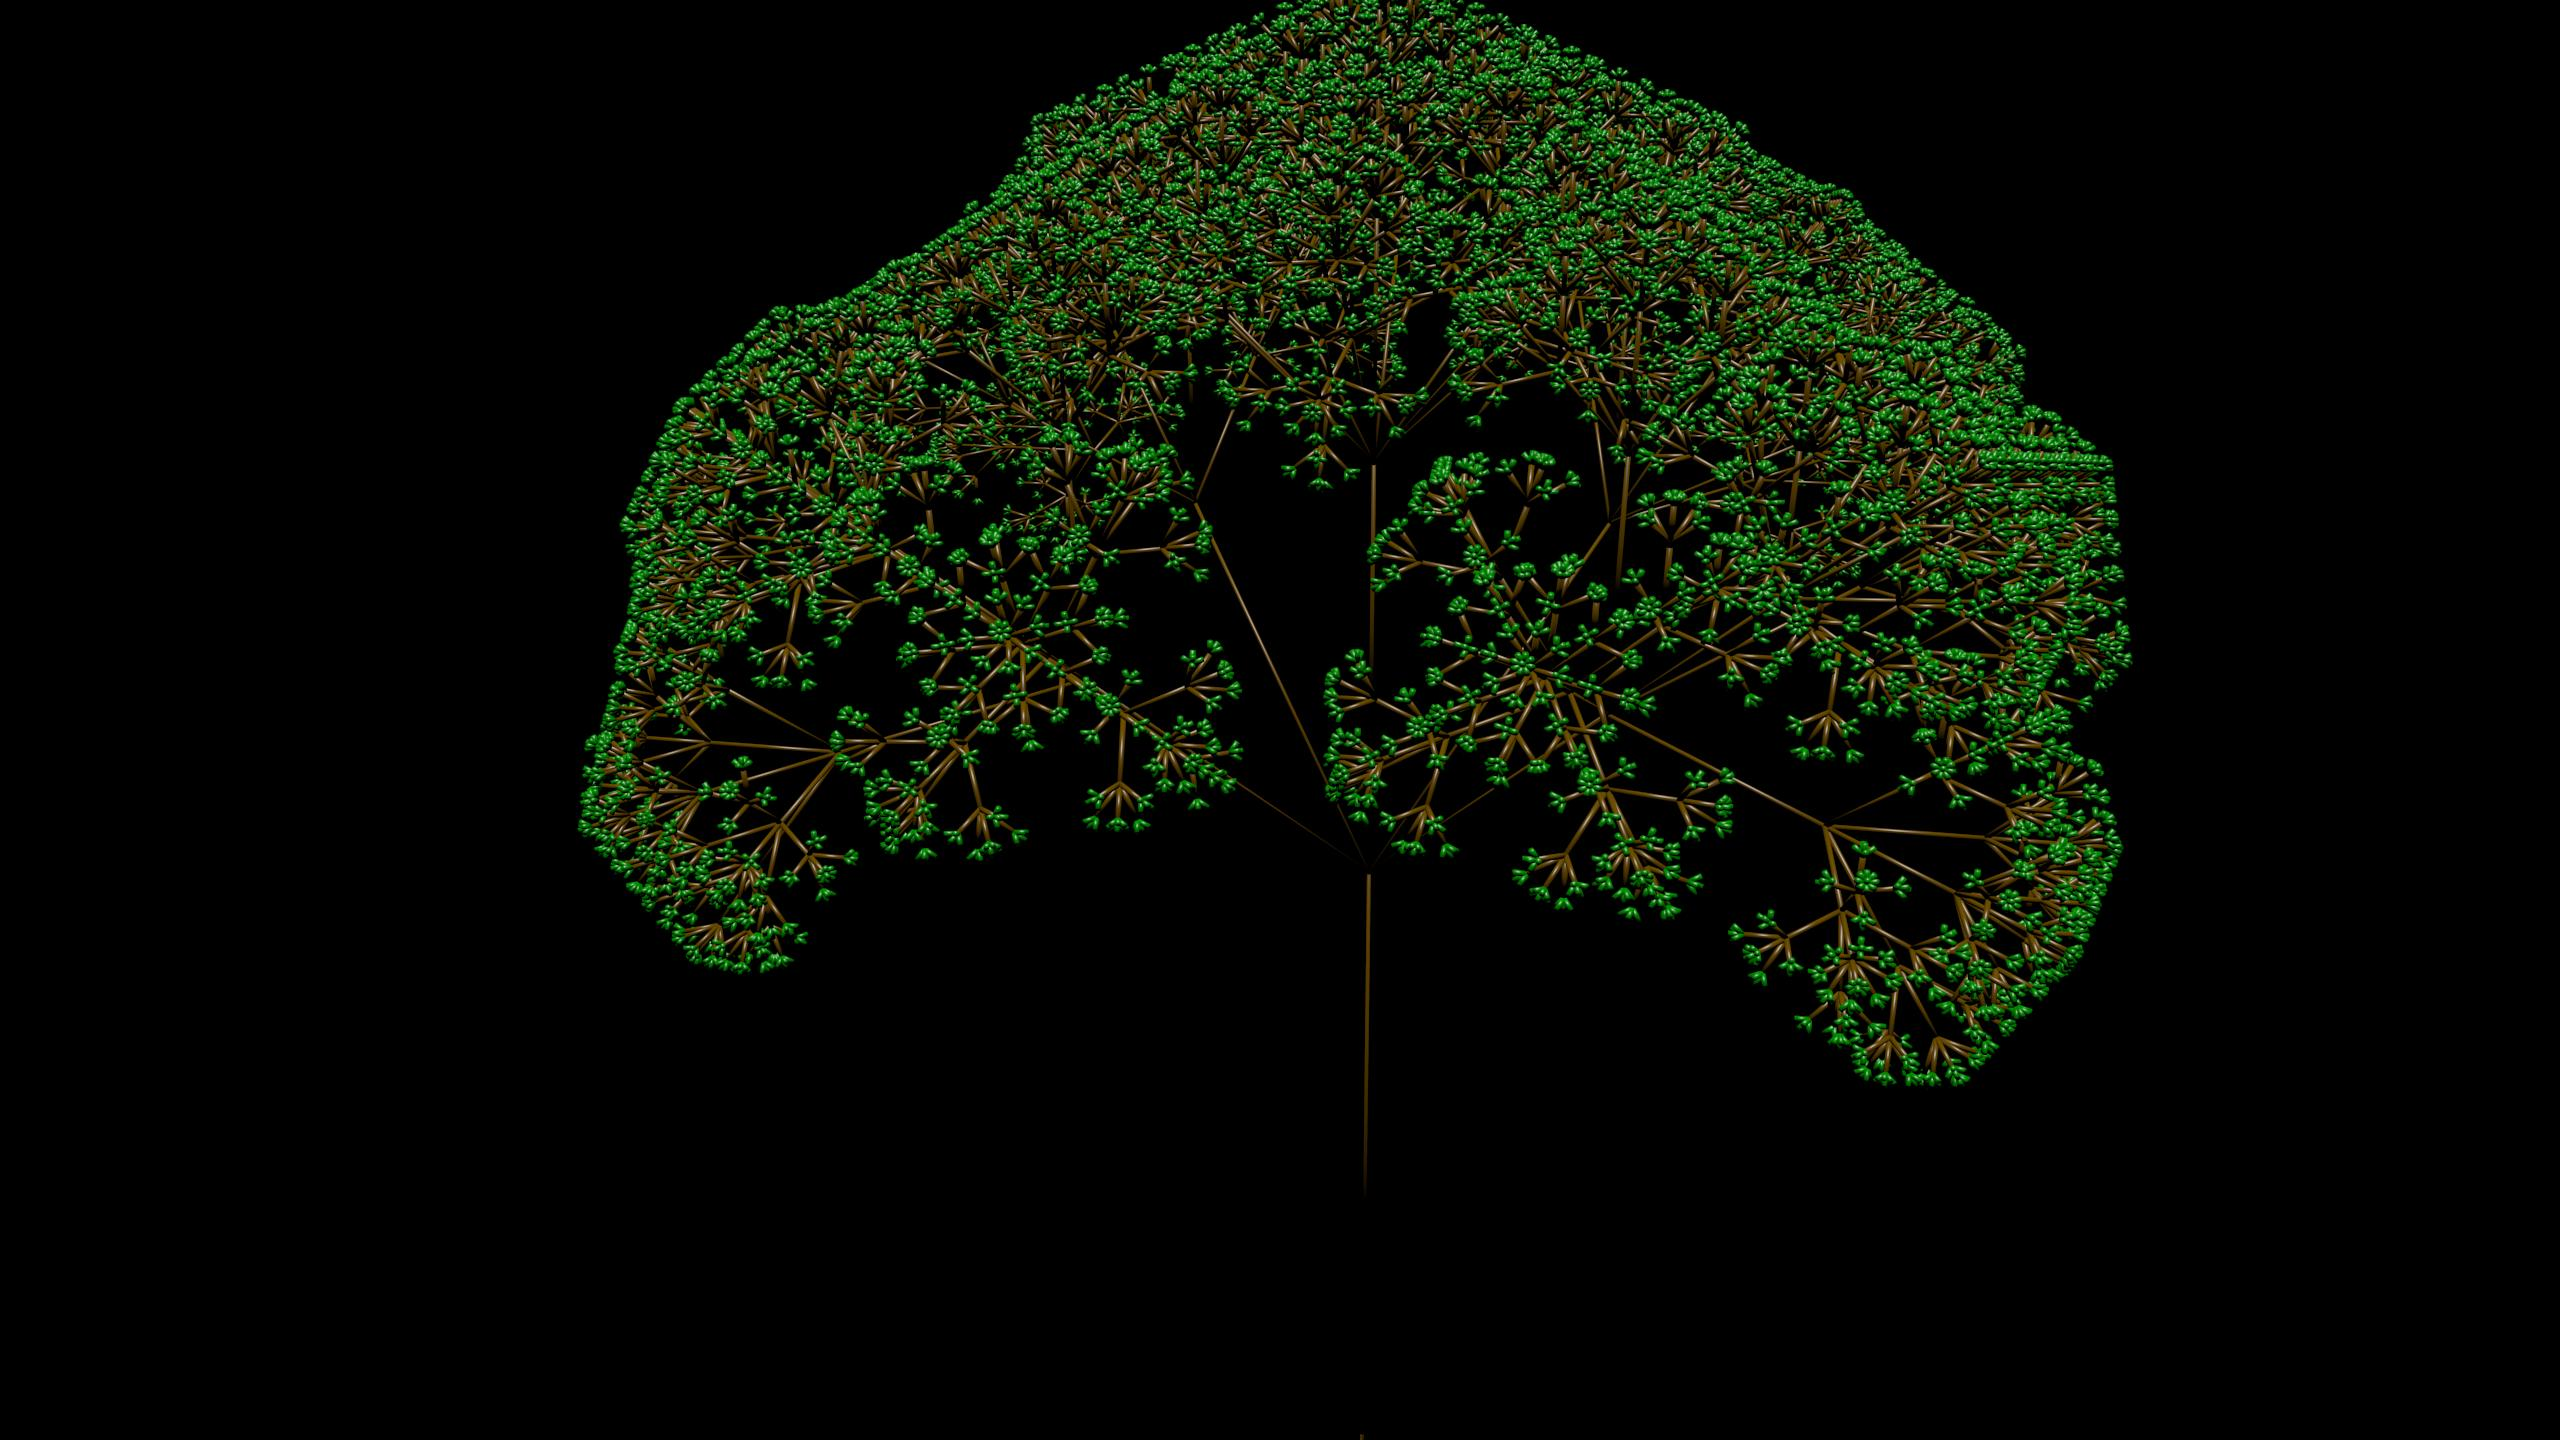
\includegraphics[width=0.75\textwidth]{figures/L-systems/prob13d.jpg}
    \caption[3D Representation of Problem 1]{A 3D representation of problem 1}\label{fig:prob1_3d}
\end{figure}

We experimented further with radii proportionality and randomness but the
results didn't look as good. Radii proportionality did not look good as a
locked radii and would probably be better if done with a function instead of a
scaler. Randomness broke the fractal nature of the designs. We found that there
were many cases where patterns would loop back on themselves and generate
multiple identical cylinders. Applying the perturbation to angle or length
resulted in a complete breakdown of the fractal symmetry. It is possible that
some simple L-System variations may have looked better but we did not find one.

% \todoinline[caption=Further extending the L-System]{Discuss how to add color, radii proportionality, and randomness}
% \todoinline[caption=Add randomness]{
%     Implement randomness.
%     I can think of two ways to do so:
%     First, add an \texttt{r} command that perturbs the immediately following command.
%     This would introduce randomness, but at regular intervals.

%     Second, add a randomness parameter to the constructor, so that if it's set, apply perturbations at random.

%     Mention that adding randomness breaks fractals with backtracking.
% }

\subsection{Implementation}\label{sec:l-sys-implementation}
Implementation of this problem was done in three parts: \mintinline{text}{grammar},
\mintinline{text}{graphics}, and \mintinline{text}{turtle}.

\subsubsection{Grammar}
This section identified which symbols we would utilize as well as how it would
build the final string. Symbols were defined within a
\href{https://docs.python.org/3/library/stdtypes.html#frozenset}{frozenset}:
\mintinline{python}{symbols}. The function: \mintinline{python}{iapply} essentially
utilizes a generator to apply production rules to the \mintinline{text}{axiom} of the
given iteration.

\subsubsection{Graphics}
Graphics assigns the initial conditions specified in the JSON file.
The various function mappings are assigned such as:

\begin{minted}{python}
self.mappings = {"F": self.turtle.move, "^": self.turtle.pitch}
\end{minted}

We then iterate through the string (\mintinline{python}{commands}), applying the
appropriate mappings. We keep track of consecutive move commands to determine
segment length. This serves to reduce the number of cylinders we have to draw
and it allows us to assign a color scheme based on length.

Cylinders are saved in a dictionary format:
\begin{minted}{python}
    cylinders.append(
        {
            "from": start,
            "to": end,
            "radius": self.radius,
            "material": "Branch" if length > 1 else "Leaf",
            "length": length,
        }
    )
\end{minted}

\begin{table}[H]
    \centering
    \caption{Dictionary of Cylinders}\label{table:dict_cylinders}
    \begin{tabular}{@{}ll@{}}
        \toprule
        \textbf{Name} & \textbf{Description}               \\ \midrule
        from          & Origin                             \\
        to            & Destination                        \\
        radius        & Radius for segment                 \\
        material      & Branch or Leaf dependent on length \\
        length        & Cylinder length                    \\ \bottomrule
    \end{tabular}
\end{table}

\autoref{table:dict_cylinders} defines what each attribute in a cylinder
means. Due to the quirks of Blender we determined it was better to create a
single cylinder and then copy it, so for each length we generate a master. The
master is copied for each cylinder of the same length, while the copy has the
appropriate \mintinline{python}{from - to} applied. This application is done through the
\mintinline{python}{draw} function. We started to have \mintinline{text}{axioms} that
were hundreds of thousands of characters long. Speed became an issue with
sufficient iterations so we developed a batch system.  We specify the number of
jobs we want to run on via command line:

\mintinline{shell}{./batch.sh data/b3d.json --jobs 32}

Essentially this chops up the \mintinline{text}{cylinders} list into 32 pieces and runs
them concurrently. Runtimes went from 45 minutes to a few seconds. The
batch process fires up \mintinline{text}{--jobs N} instances of Blender. This can
quickly consume all RAM. We had to play around with the limits of our
individual machines to find the maximums. This batch process allowed us to
break 19,000 cylinders which was a hard threshold we were struggling to surpass.
We were able to generate over 400,000 cylinders without issue utilizing the
batch method.

Individually generated \mintinline{text}{.blend} files are joined into a
single entity which reduces the size of the stored 3D object. If the resulting
\mintinline{text}{.fbx} file is under 50MB we were able to upload it to
\href{https://sketchfab.com/macattackftw/models}{Sketchfab}.

\subsubsection{Turtle}
The turtle is a very simple python class. Blender's mintinline{python}{mathutils} library makes turtles
very easy to implement. Prior to finding this we spent several days trying to
get Quaternions working. The \mintinline{python}{turtle} class only has a few
functions:

\begin{itemize}
    \item push
    \item pop
    \item move
    \item roll
    \item pitch
    \item yaw
    \item position
\end{itemize}

Roll, pitch, and yaw are simply matrix multiplications applied to the existing
rotation. Move is a matrix multiplication applied to the existing position.
Push and pop are utilized for setting and then returning to that position
respectively.

% \todoinline{
%     McGough has seemed to like my (brief) discussion of my previous implementations.
%     We should not give the whole thing, just the interesting bits and pieces.
% }

\subsubsection{Existing Implementations}
There are a number of existing implementations for Lindenmayer Systems in Python --- at least one of which is even done in three dimensions.

The first implementation of L-Systems that we found was actually a \LaTeX{} Tikz implementation.
It's quite easy to use.
\autoref{fig:latex-lsystem} shows the result of the Tikz code shown in \autoref{code:latex-lsystem}.

\begin{figure}[H]
    \centering

    \pgfdeclarelindenmayersystem{Fractal plant}{
    \rule{X -> F-[[X]+X]+F[+FX]-X}
    \rule{F -> FF}
    }

    \begin{tikzpicture}
        \draw [green!50!black, rotate=90][
            l-system={
                    Fractal plant,
                    axiom=X,
                    order=5,
                    step=2pt,
                    angle=25
                }
        ] lindenmayer system;
    \end{tikzpicture}
    \caption{A fractal plant generated with \LaTeX}\label{fig:latex-lsystem}
\end{figure}

\begin{listing}[H]
    \begin{minted}{latex}
        \documentclass[tikz, border=1mm]{standalone}

        \usetikzlibrary{lindenmayersystems}

        \pgfdeclarelindenmayersystem{Fractal plant}{
            \rule{X -> F-[[X]+X]+F[+FX]-X}
            \rule{F -> FF}
        }

        \begin{document}
        \begin{tikzpicture}
            \draw [green!50!black, rotate=90][
                l-system={
                        Fractal plant,
                        axiom=X,
                        order=5,
                        step=2pt,
                        angle=25
                    }
            ] lindenmayer system;
        \end{tikzpicture}
        \end{document}
    \end{minted}
    \caption{A fractal plant with \LaTeX}\label{code:latex-lsystem}
\end{listing}

We also found numerous 2D Python implementations. Some of which are listed below, ranked by their usefulness.
\begin{enumerate}
    \item \href{http://www.4dsolutions.net/ocn/lsystems.html}{4dsolutions}
    \item \href{https://hackaday.io/project/11721-python-l-system}{Hackaday project}
    \item \href{https://interactivepython.org/courselib/static/thinkcspy/Strings/TurtlesandStringsandLSystems.html}{How To Think Like A Computer Scientist project}
\end{enumerate}

The original paper \textit{The Algorithmic Beauty of Plants} can be found online at \url{http://algorithmicbotany.org/papers/\#abop}.

The original idea to make a variant of the Lindenmayer system in three dimensions came from \href{https://stackoverflow.com/questions/42257676/l-systems-and-the-stack-in-maya}{this Stack Overflow post}.
However, in that post the author is using the Maya Python API, which has very little documentation and supporting material online.
Further, Maya is quite expensive (\$3,000+) for non-educational use, so there was little practical advantage to learning it on the side.
Thus we decided to use the free, open source modeling software \href{https://www.blender.org/}{Blender}.

Blender has excellent mathematics libraries for performing 3D graphics manipulation, which was exactly what we wanted for this project.
We spent roughly a week before another round of Googling produced the \href{https://github.com/lemurni/lpy-lsystems-blender-addon}{Lindenmaker Blender addon}.
Lindenmaker is a Python library that adds a new panel to Blender for producing L-system trees.
Lindenmaker is the result of the bachelor's thesis available \href{https://www.cg.tuwien.ac.at/research/publications/2017/LEOPOLD-2017-ALG/LEOPOLD-2017-ALG-thesis.pdf}{here}.

Due to the spirit of the assignment we decided to avoid blindly using the Lindenmaker addon without implementing our own solution.
However, we still took inspiration from Lindenmaker's implementation of the 3D turtle because we struggled getting quaternion transformations to apply to each object's \textit{local} reference frame.

\subsubsection{Computing the Vertices}
I have no clue what kind of voodoo mathamagic you used to do this.
\todoinline[caption=Implementation of the vertex computation]{
    Discuss the \mintinline{python}{Graphics.compute(lstring)} method and its implementation.
    Be sure to include the data structure it returns and how the material is set.

    Also include the proportional radii, and randomness (once it's implemented).
}

% \subsubsection{Adding Cylinders to the 3D Scene}
% Covered in Graphics subsubsection. I don't think he cares about the details that much in regards to Blender.
% \todoinline[caption=Implementation of adding objects to the scene]{
%     Show how to add a single cylinder to the scene, and mention that it slowed down Blender substantially.

%     Show how to fix this by duplicating cylinders, but mention that there was still a substantial slowdown for large fractals.
% }

% \subsubsection{Parallel Scene Creation}
% He's not going to care about the code to join blender files, though the process is explained above.
% \todoinline[caption=Implementation of batch processing]{
%     Discuss the general idea of the batch mode, but there's no need to give actual code --- other than how to join two files.
% }

\subsubsection{Usage}
We initially designed this to be ran in a single thread with no concurrent
usage. This proved inadequate for sufficiently large L-Systems. The recommended
mode of operation is batch and to do so simply generate a JSON file in
the format shown in \autoref{code:prob1_json}. Save the file
in whatever folder you wish, then run:

\mintinline{shell}{./batch.sh data/myJSON.json --jobs N}

To keep things neat we recommend placing the JSON file in the data
folder. Jobs (\mintinline{text}{N}) can be from 1 to as much RAM as your system can
handle. It is not recommended to go beyond 32 jobs unless you have more than
16GB of RAM.

The final file will be \mintinline{text}{data/myJSON.blend}. All of the
\mintinline{text}{myJSON-job-*-.blend} are from the \mintinline{text}{N} jobs scheduled and are the
individual components of the final \mintinline{text}{.blend} file.

% \todoinline[caption=Script usage]{
%     Discuss how to use each of the scripts we created, spending the most time on \texttt{blender.py} and \texttt{batch.sh}.

%     Make sure to point out that the \mintinline{python}{bpy} and \mintinline{python}{mathutils} libraries are provided by Blender, and that to use them we need to run our scripts in funky ways.
% }

\subsection{Results}
Results of Problem one can be seen in \autoref{fig:prob1_45},
\autoref{fig:prob1_90}, and \autoref{fig:prob1_120}. The \mintinline{text}{.fbx} files can be
found on
\href{https://sketchfab.com/macattackftw/collections/problem-1}{Sketchfab}.

\begin{figure}[H]
    \centering
    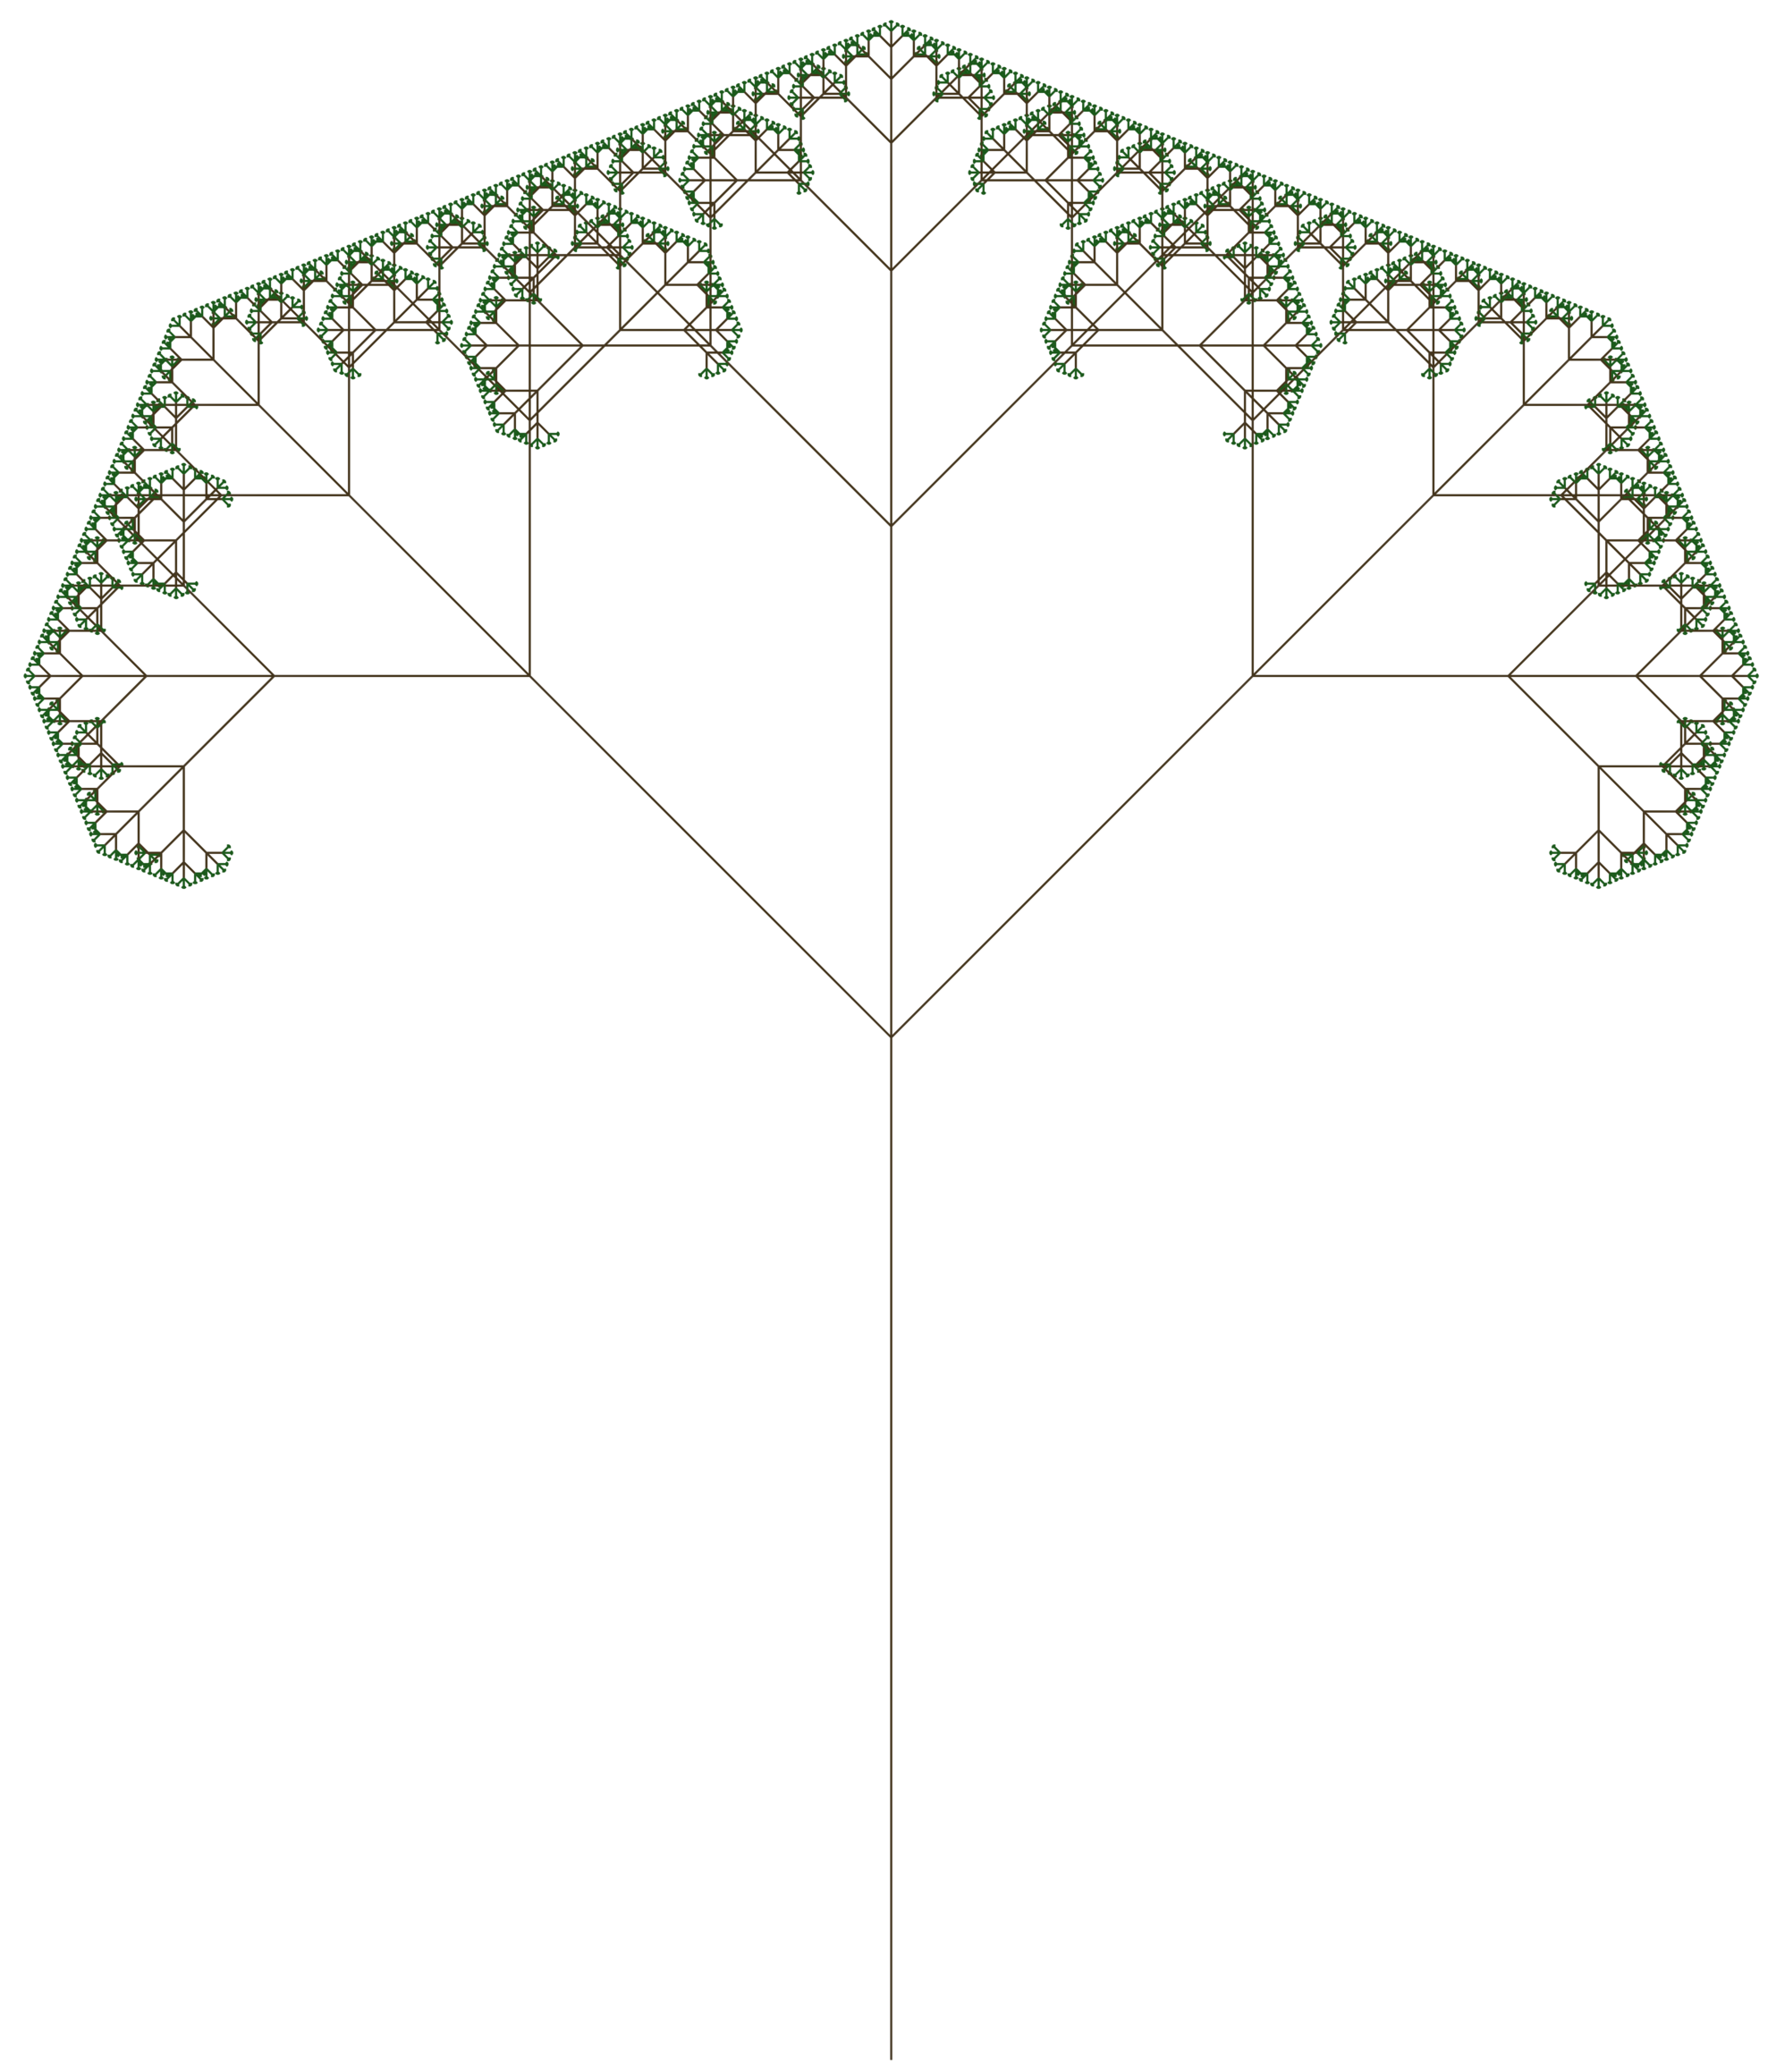
\includegraphics[width=0.75\textwidth]{figures/L-systems/prob1-45}
    \caption{Problem 1 where $\theta = 45^\circ$}\label{fig:prob1_45}
\end{figure}

\begin{figure}[H]
    \centering
    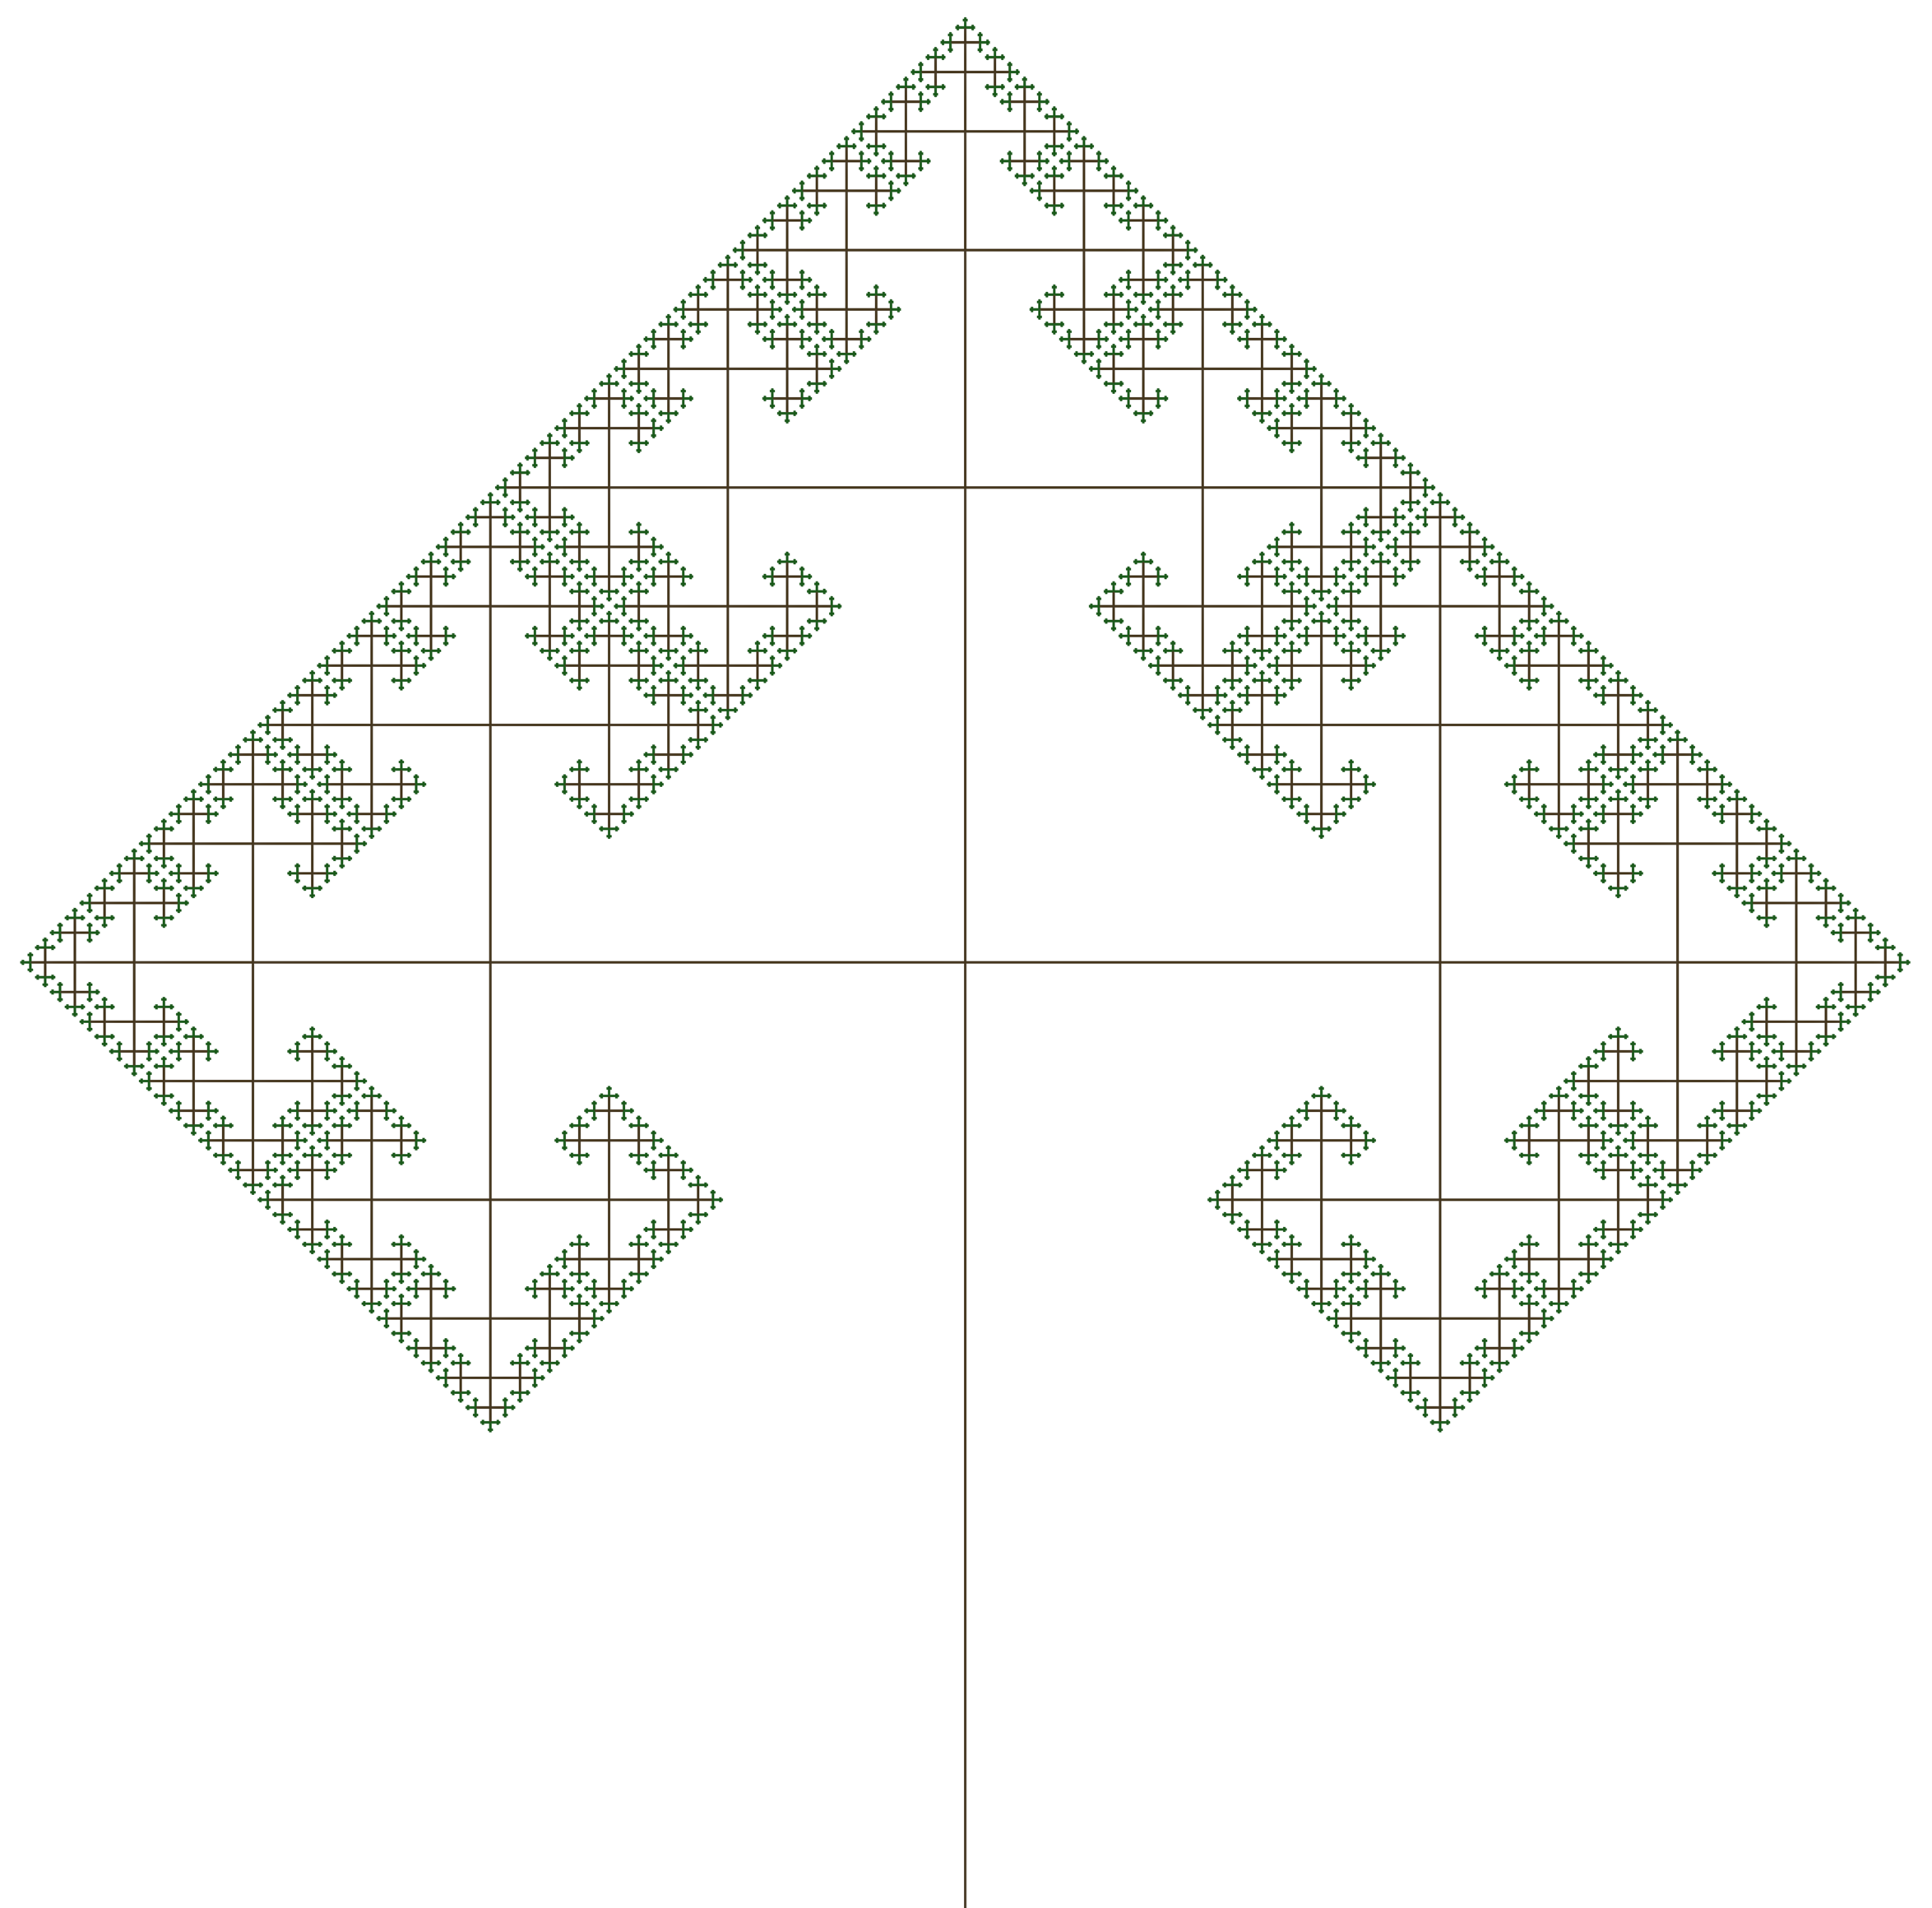
\includegraphics[width=0.75\textwidth]{figures/L-systems/prob1-90}
    \caption{Problem 1 where $\theta = 90^\circ$}\label{fig:prob1_90}
\end{figure}

\begin{figure}[H]
    \centering
    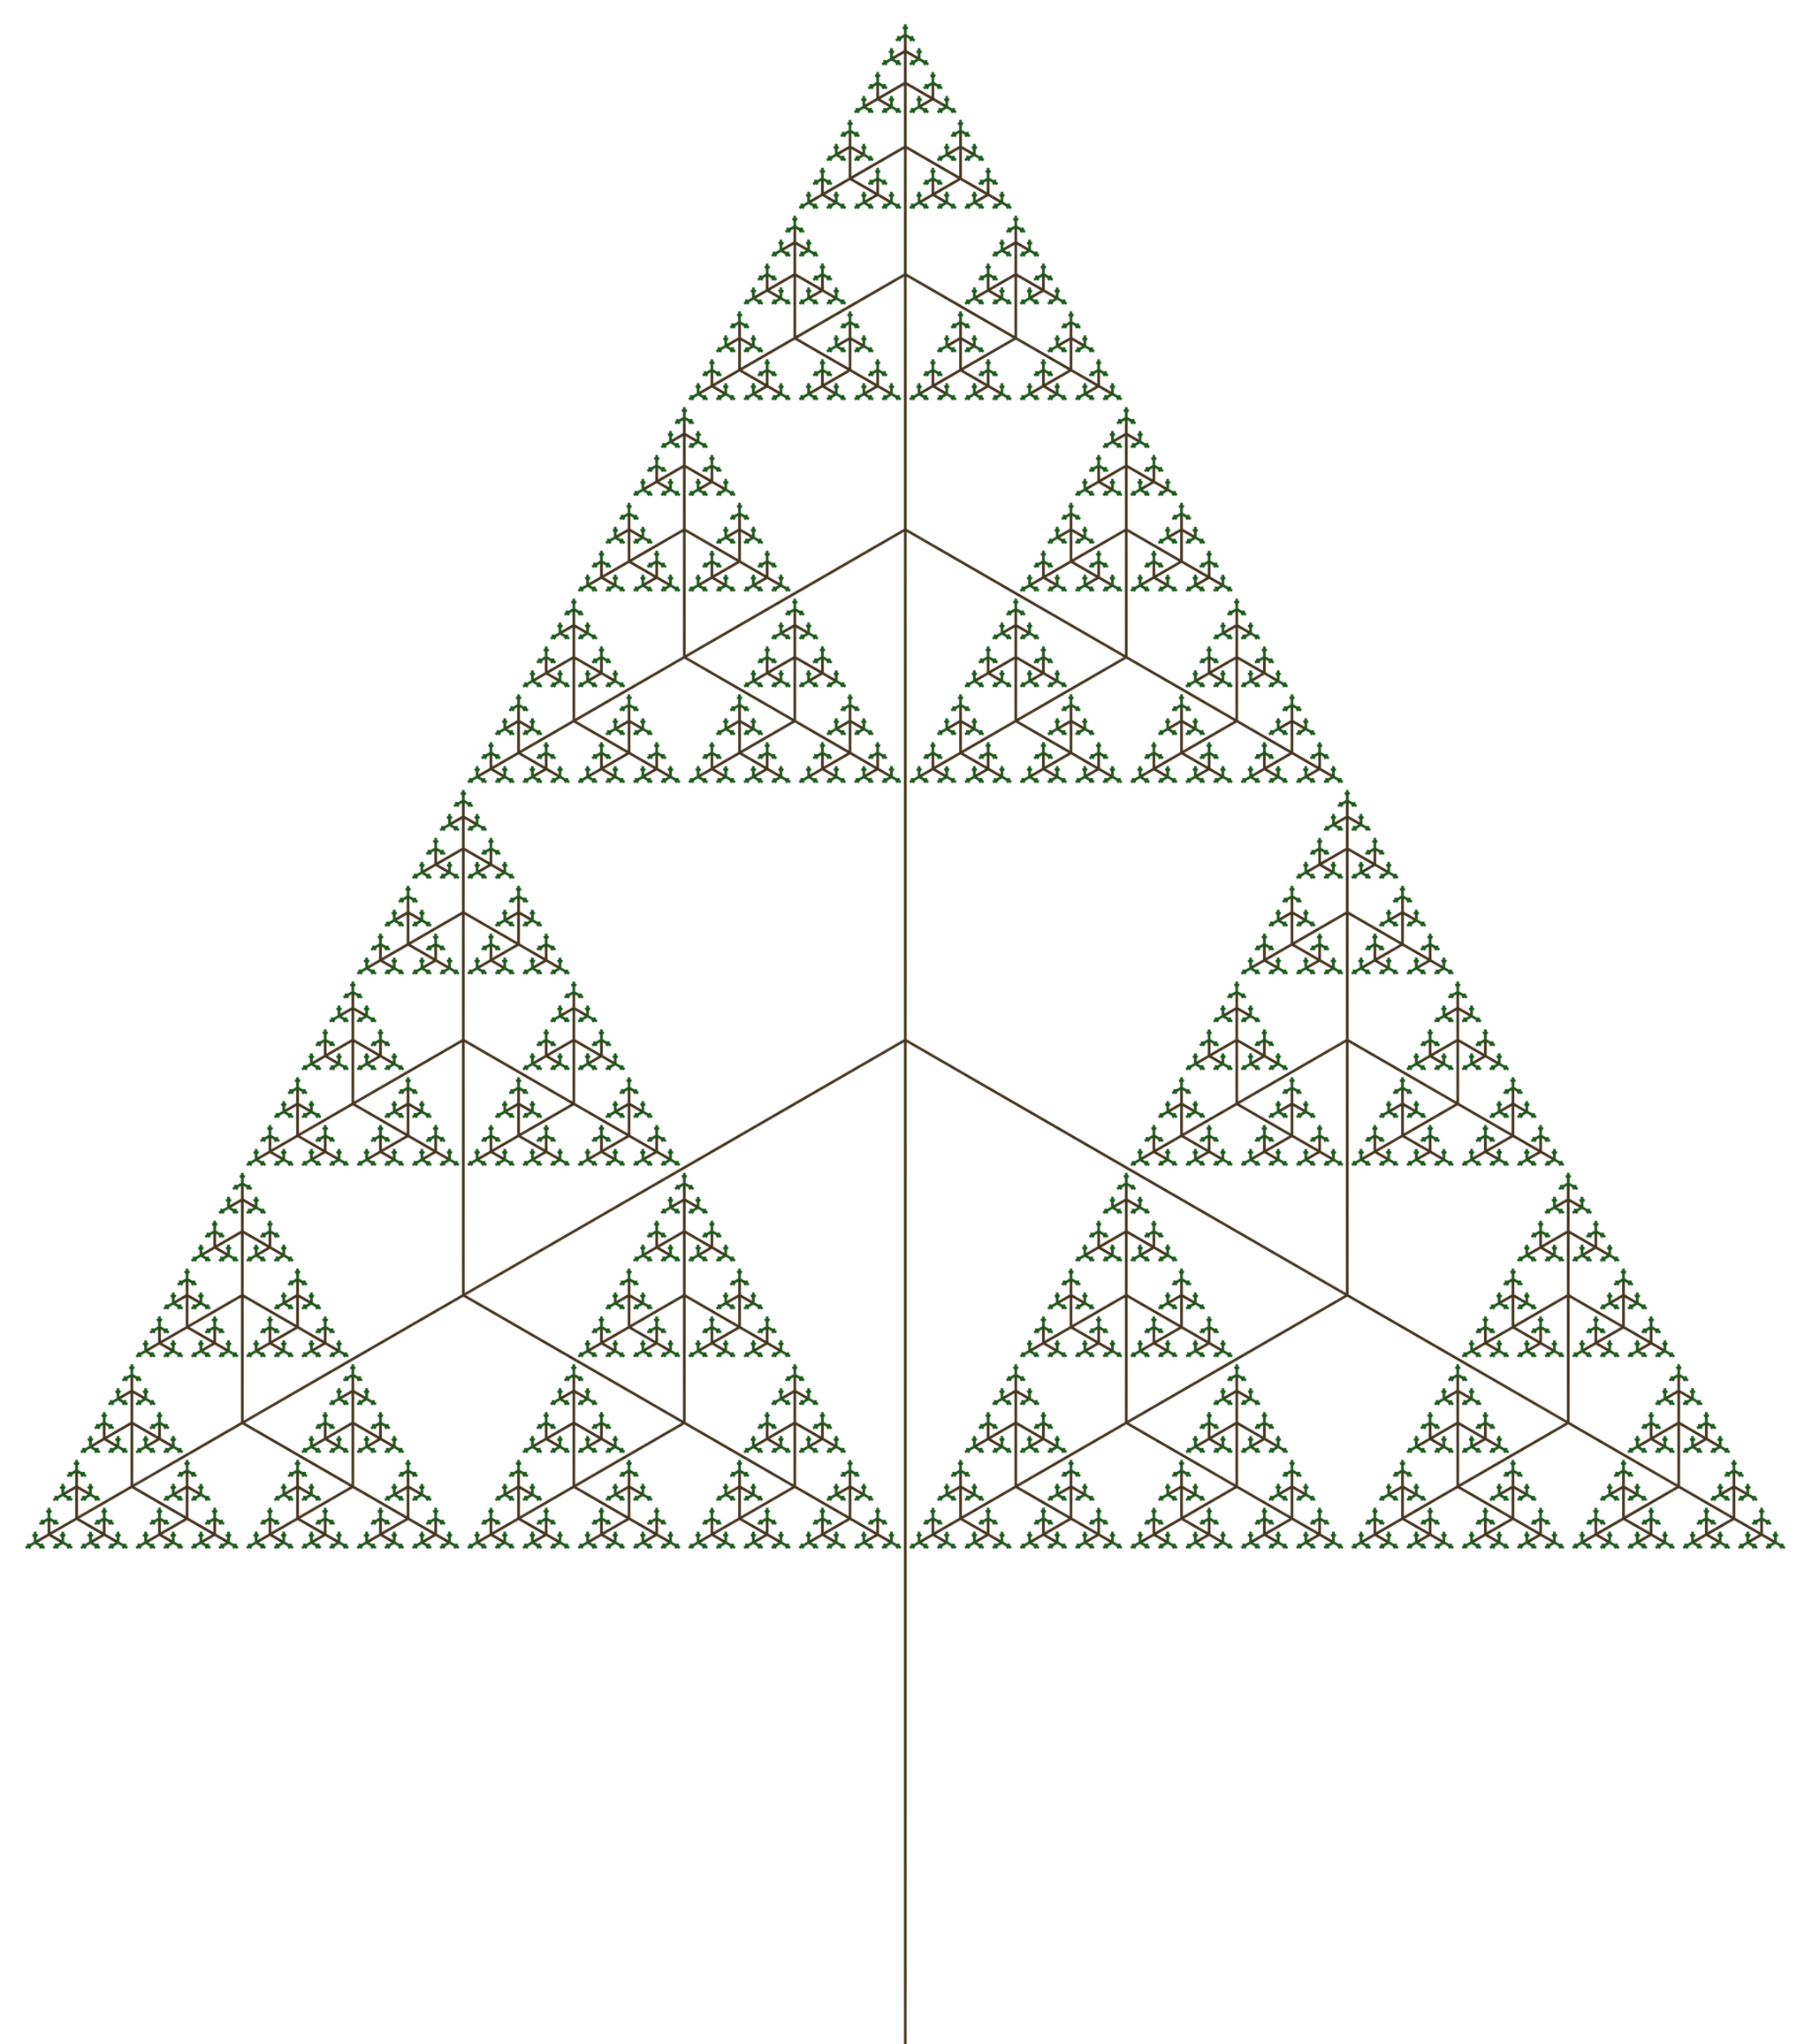
\includegraphics[width=0.75\textwidth]{figures/L-systems/prob1-120}
    \caption{Problem 1 where $\theta = 120^\circ$}\label{fig:prob1_120}
\end{figure}

% \subsubsection{The Lindenmayer System for the Given Problem}
% \todoinline[caption=results for given problem]{
%     Show our results for the given problem.

%     Show the production rules, and generated graphics.
%     Play with the scale and the yaw angle.
% }

% \todoinline[caption=Move experimentation to problem 2]{
%     Leave the 3D and other experimentation to problem 2, because it asks you to experiment, and we can get more mileage out of it there.
% }

\subsection{Conclusion}
L-Systems are great for generation of interesting fractal patterns. We
generated several additional variations which can be found
\href{https://sketchfab.com/macattackftw/models}{here}. We wanted a visually
appealing implementation and we accomplished that. The L-System itself is
rather straightforward. Storing cylinder start/stop locations was relatively
simple, the bulk of our work was spent on visualizing and optimizing to work
with Blender. While that was not the goal of the problem it was useful to
experiment with an unfamiliar API and integrate our product with it.

There could be future work in expanding color schemes, variable radii, and
further optimizing blender usage (such as chopping up the JSON file based on
batches). We thoroughly explored L-Systems and it was a fun project.

% !TeX root = ../hw4.tex
\section{Reproducing the Book's Fractal Plants}

\subsection{Statement}
Use bracketed OL-systems to reproduce each of the plant-like fractals in Figure 7.24 of the book.

Experiment with the production rules and produce at least ten derivatives.

\subsection{Method}
The methods here are no different than Section \ref{sec:l-system-method}.

\subsection{Implementation}
The implementation is identical to Section \ref{sec:l-sys-implementation}.

\subsection{Results}\label{sec:p2-results}

\begin{figure}[H]
    \centering
    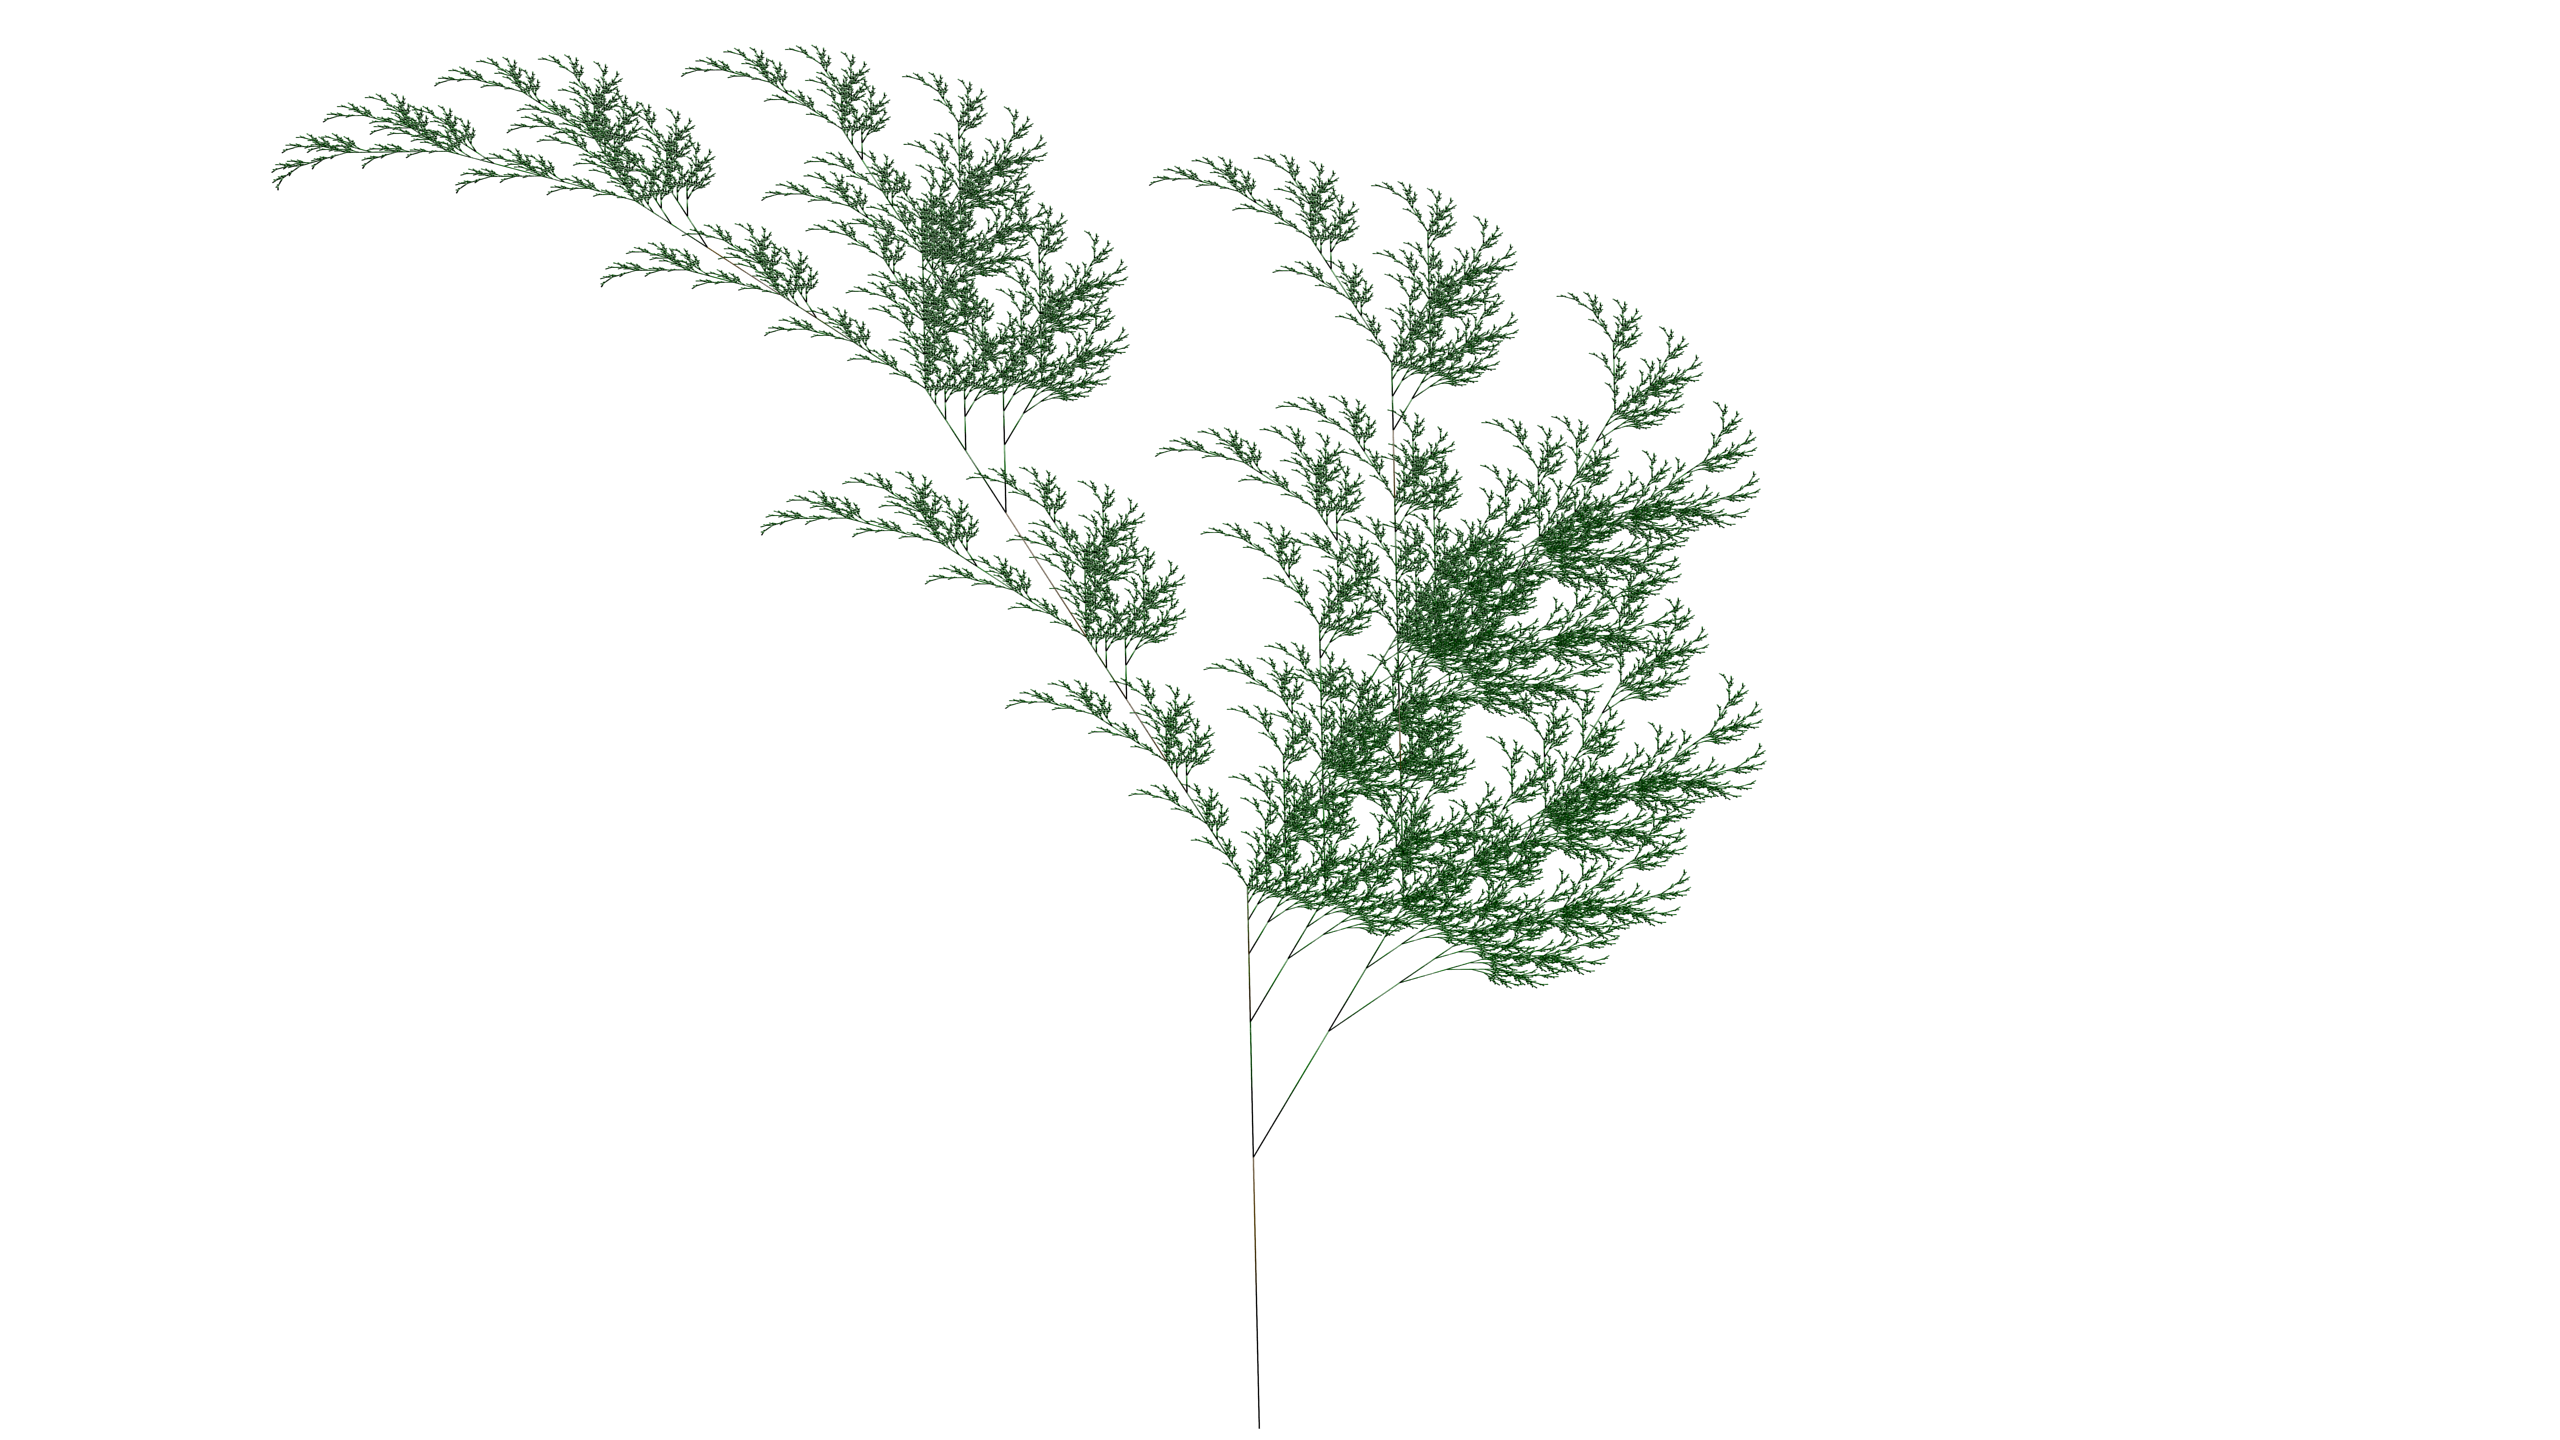
\includegraphics[width=0.90\textwidth]{figures/L-systems/a.png}
    \caption{Problem 2a}\label{fig:prob2a}
\end{figure}

\begin{figure}[H]
    \centering
    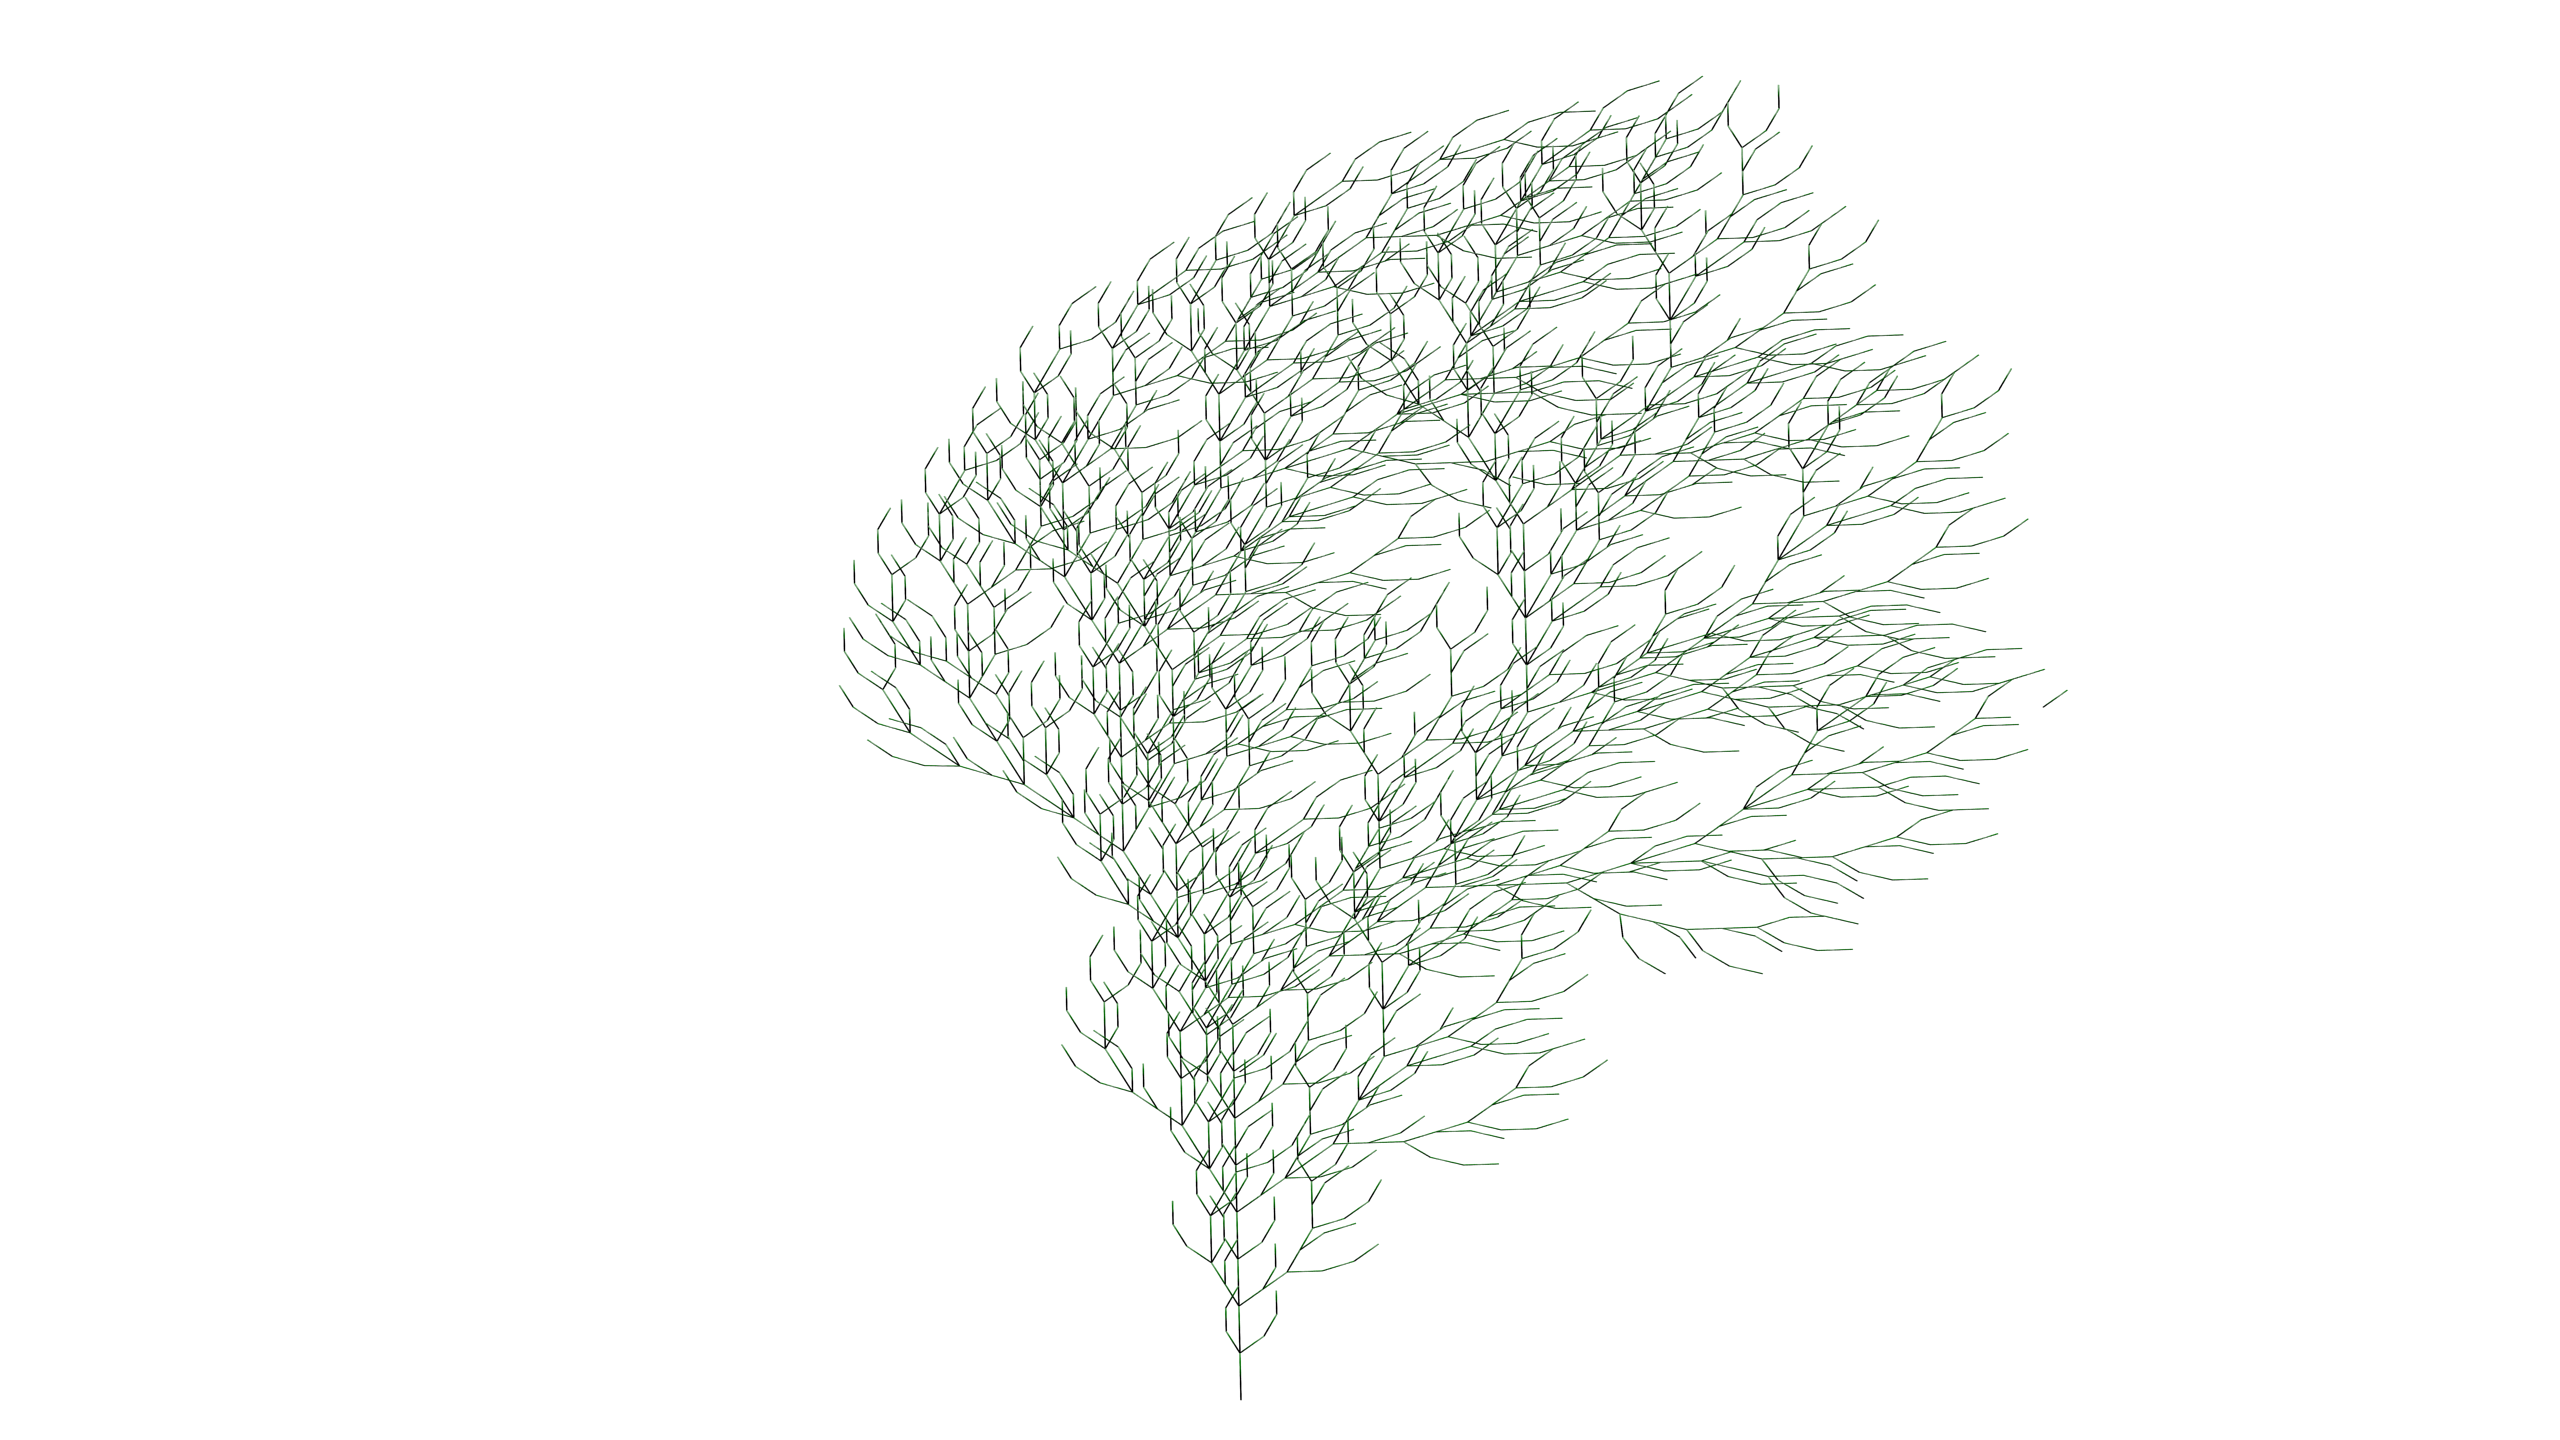
\includegraphics[width=0.90\textwidth]{figures/L-systems/b.png}
    \caption{Problem 2b}\label{fig:prob2b}
\end{figure}

\begin{figure}[H]
    \centering
    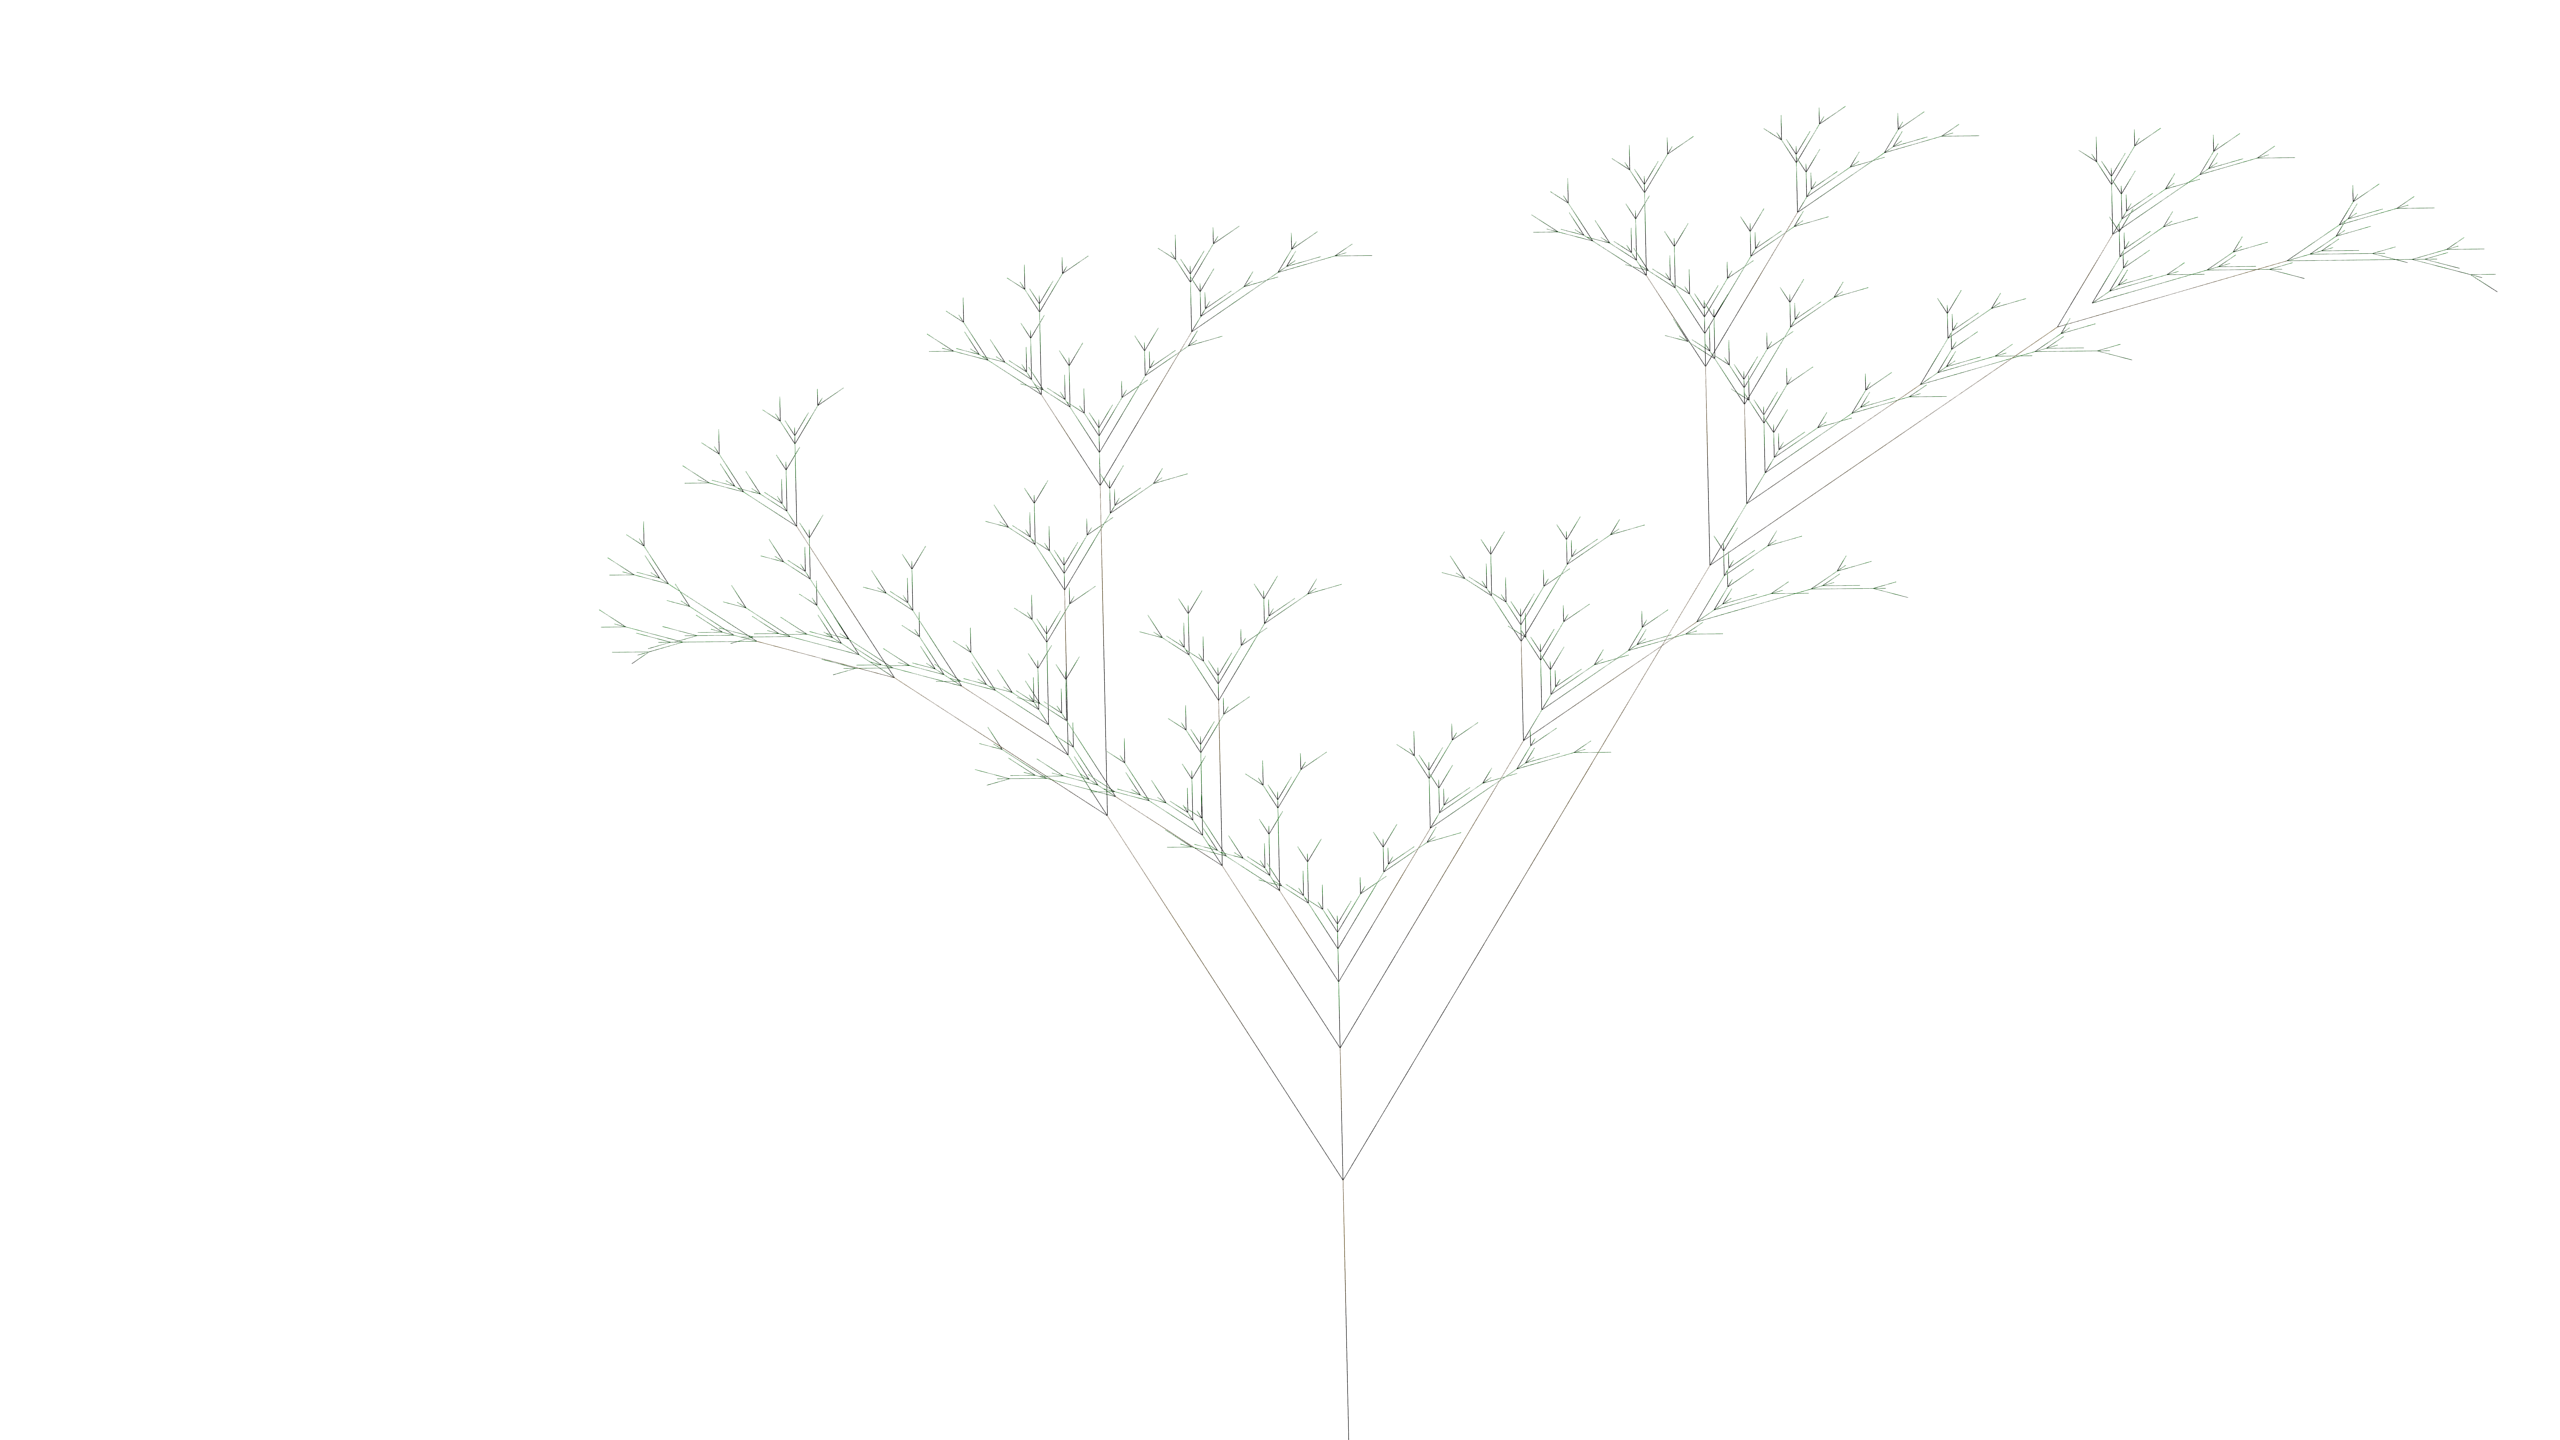
\includegraphics[width=0.90\textwidth]{figures/L-systems/c.png}
    \caption{Problem 2c}\label{fig:prob2c}
\end{figure}

\begin{figure}[H]
    \centering
    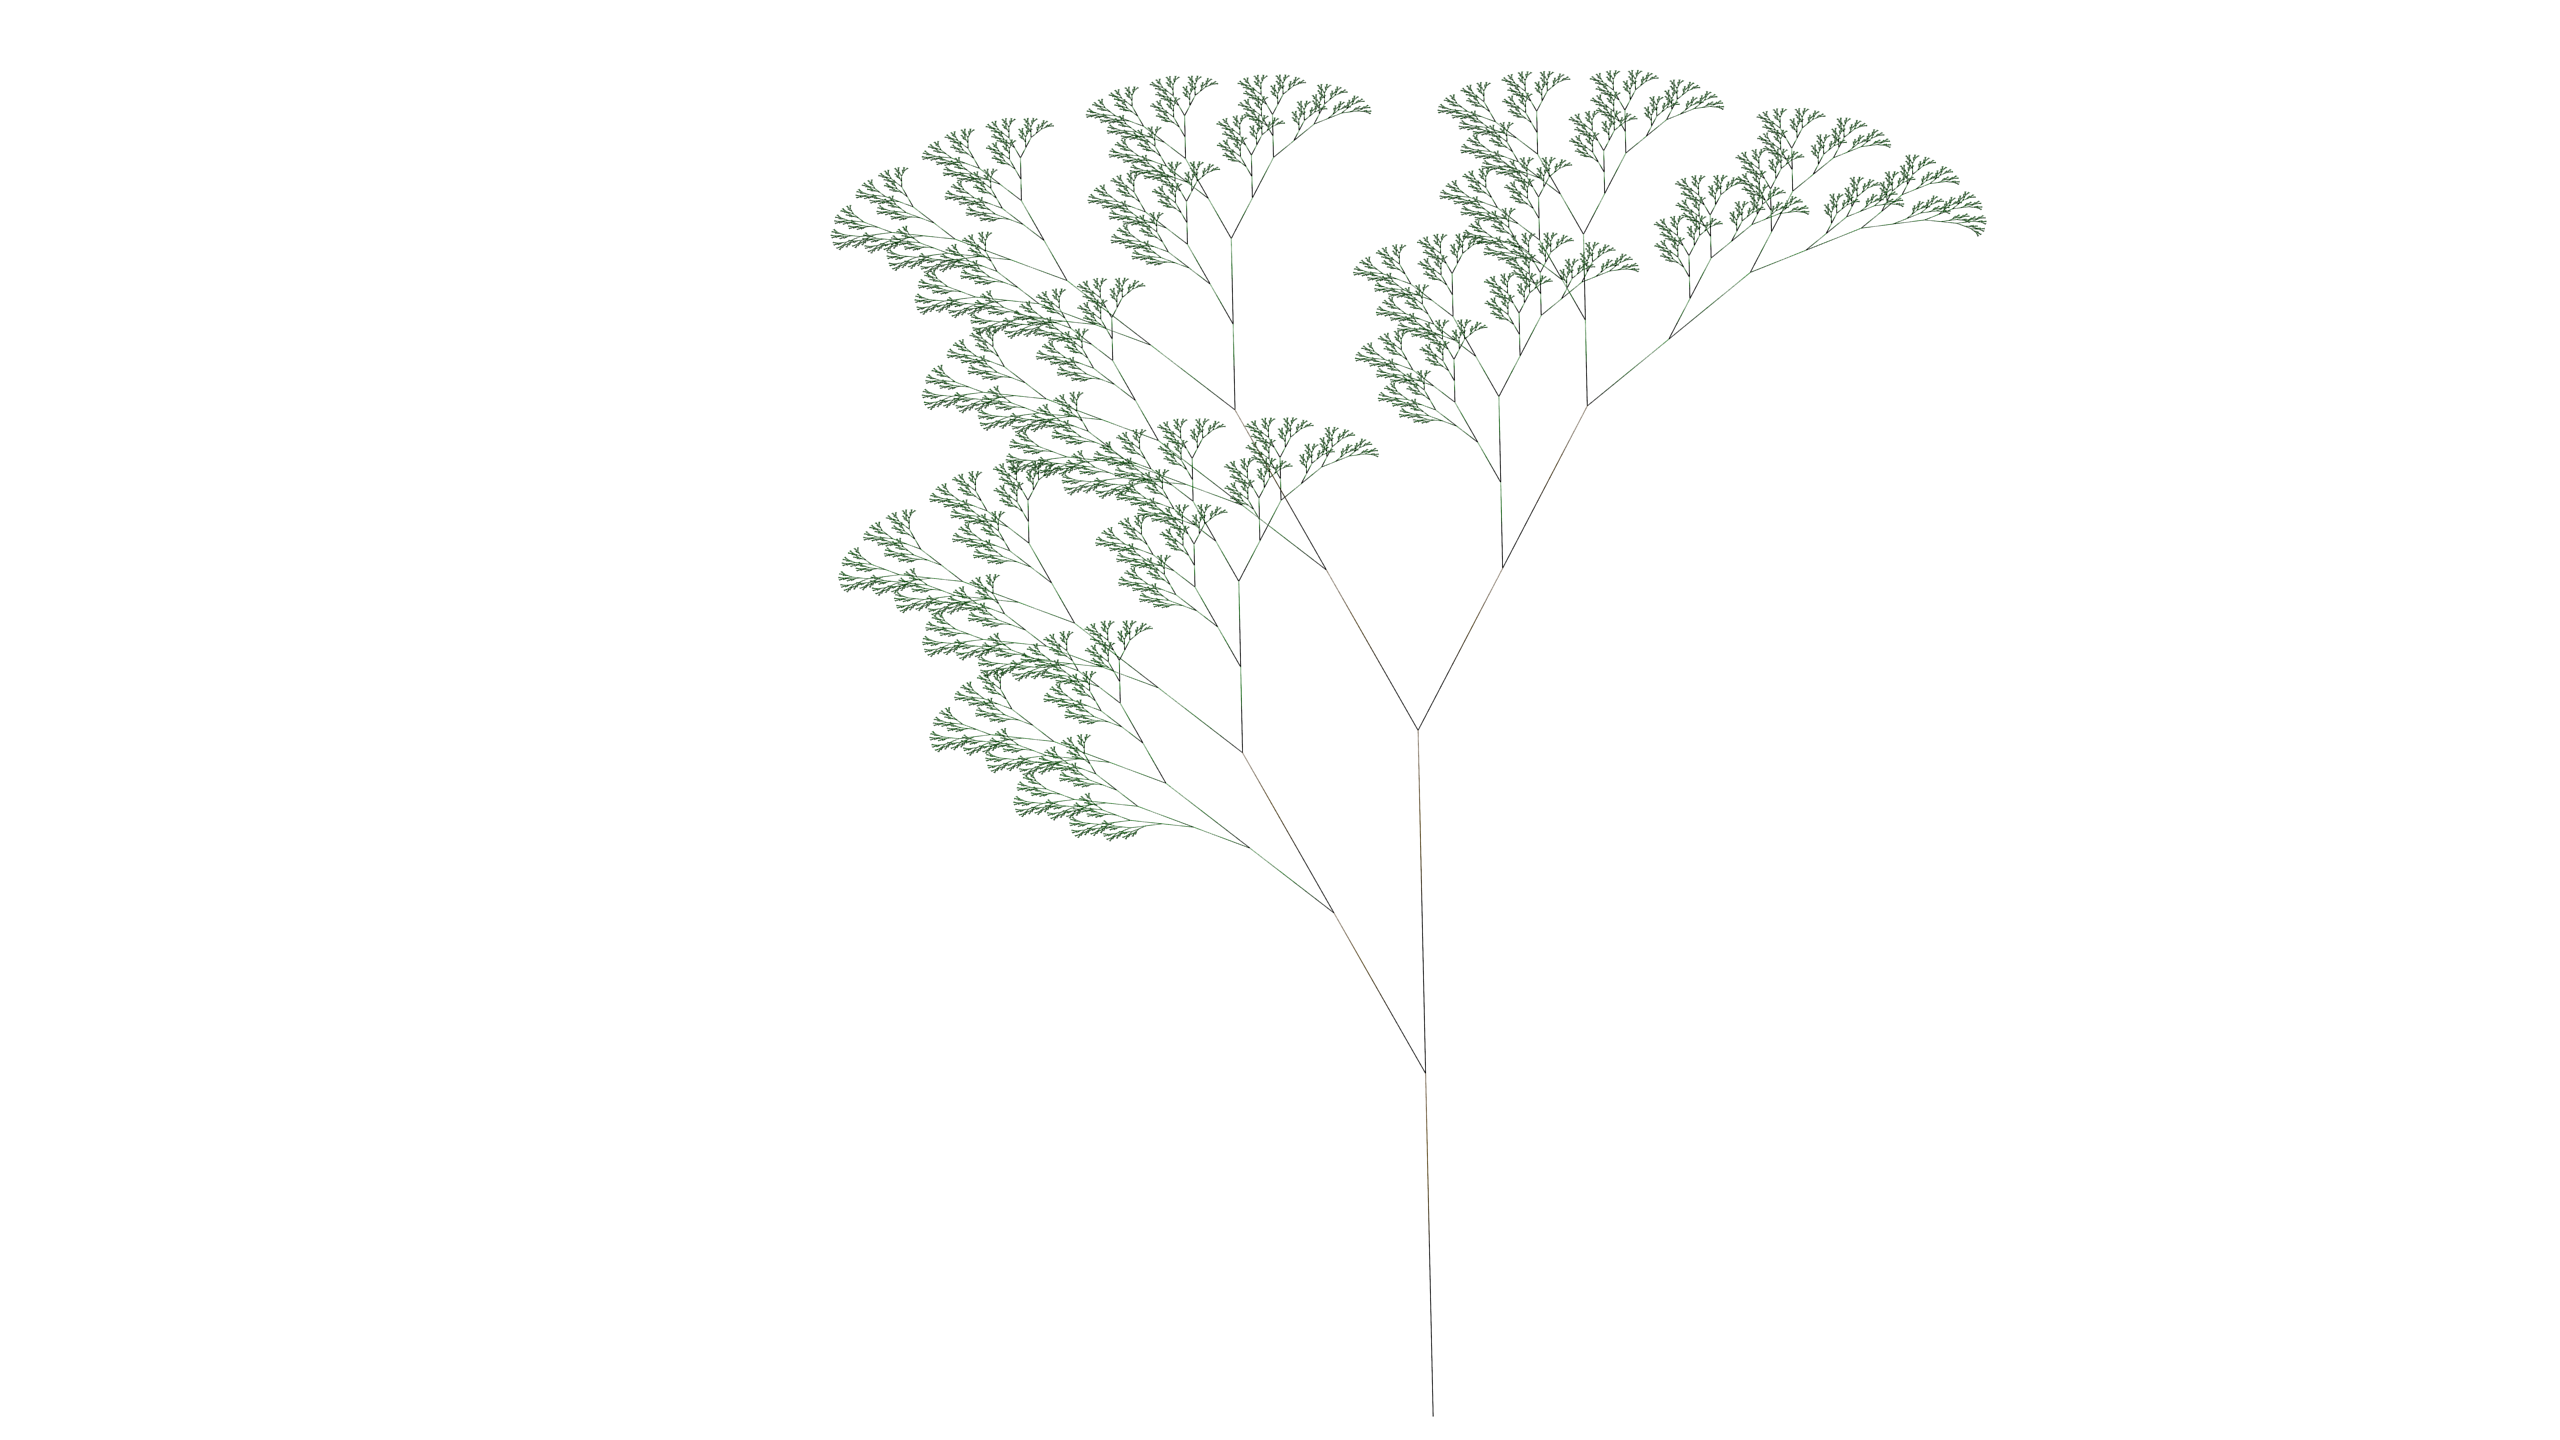
\includegraphics[width=0.90\textwidth]{figures/L-systems/d.png}
    \caption{Problem 2d}\label{fig:prob2d}
\end{figure}

\begin{figure}[H]
    \centering
    \noindent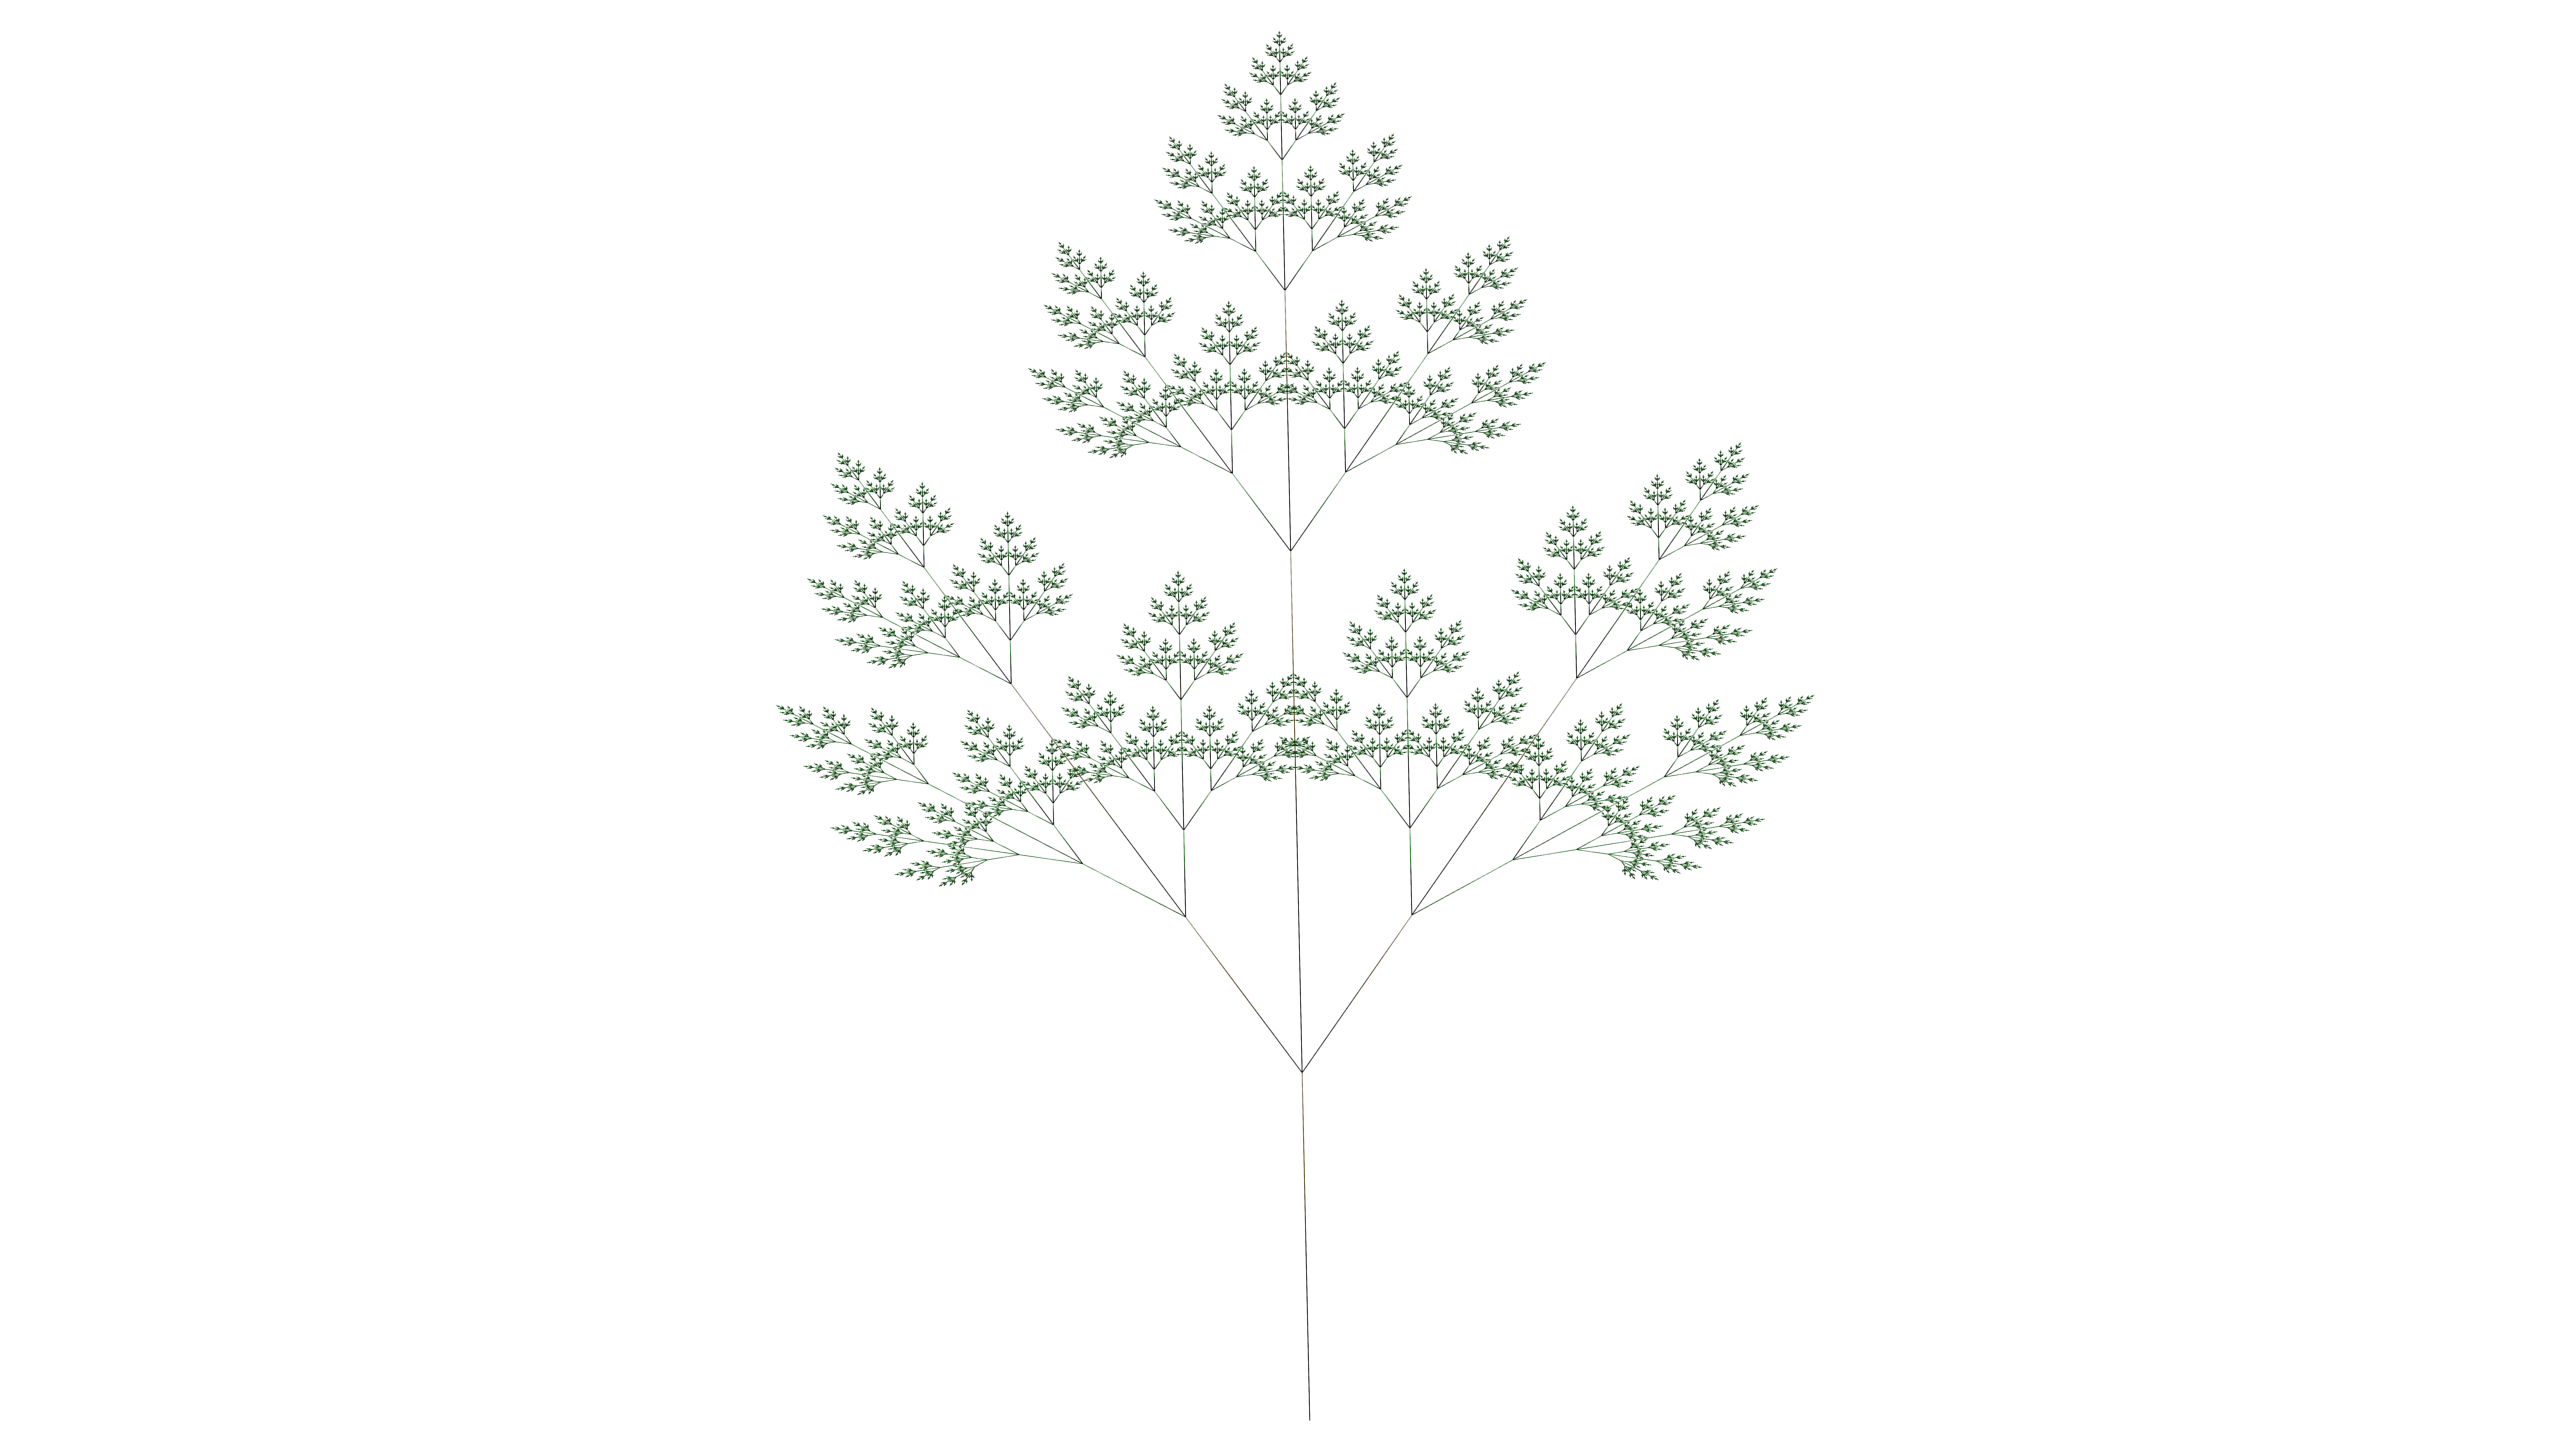
\includegraphics[width=0.90\textwidth]{figures/L-systems/e.png}
    \caption{Problem 2e}\label{fig:prob2e}
\end{figure}

\begin{figure}[H]
    \centering
    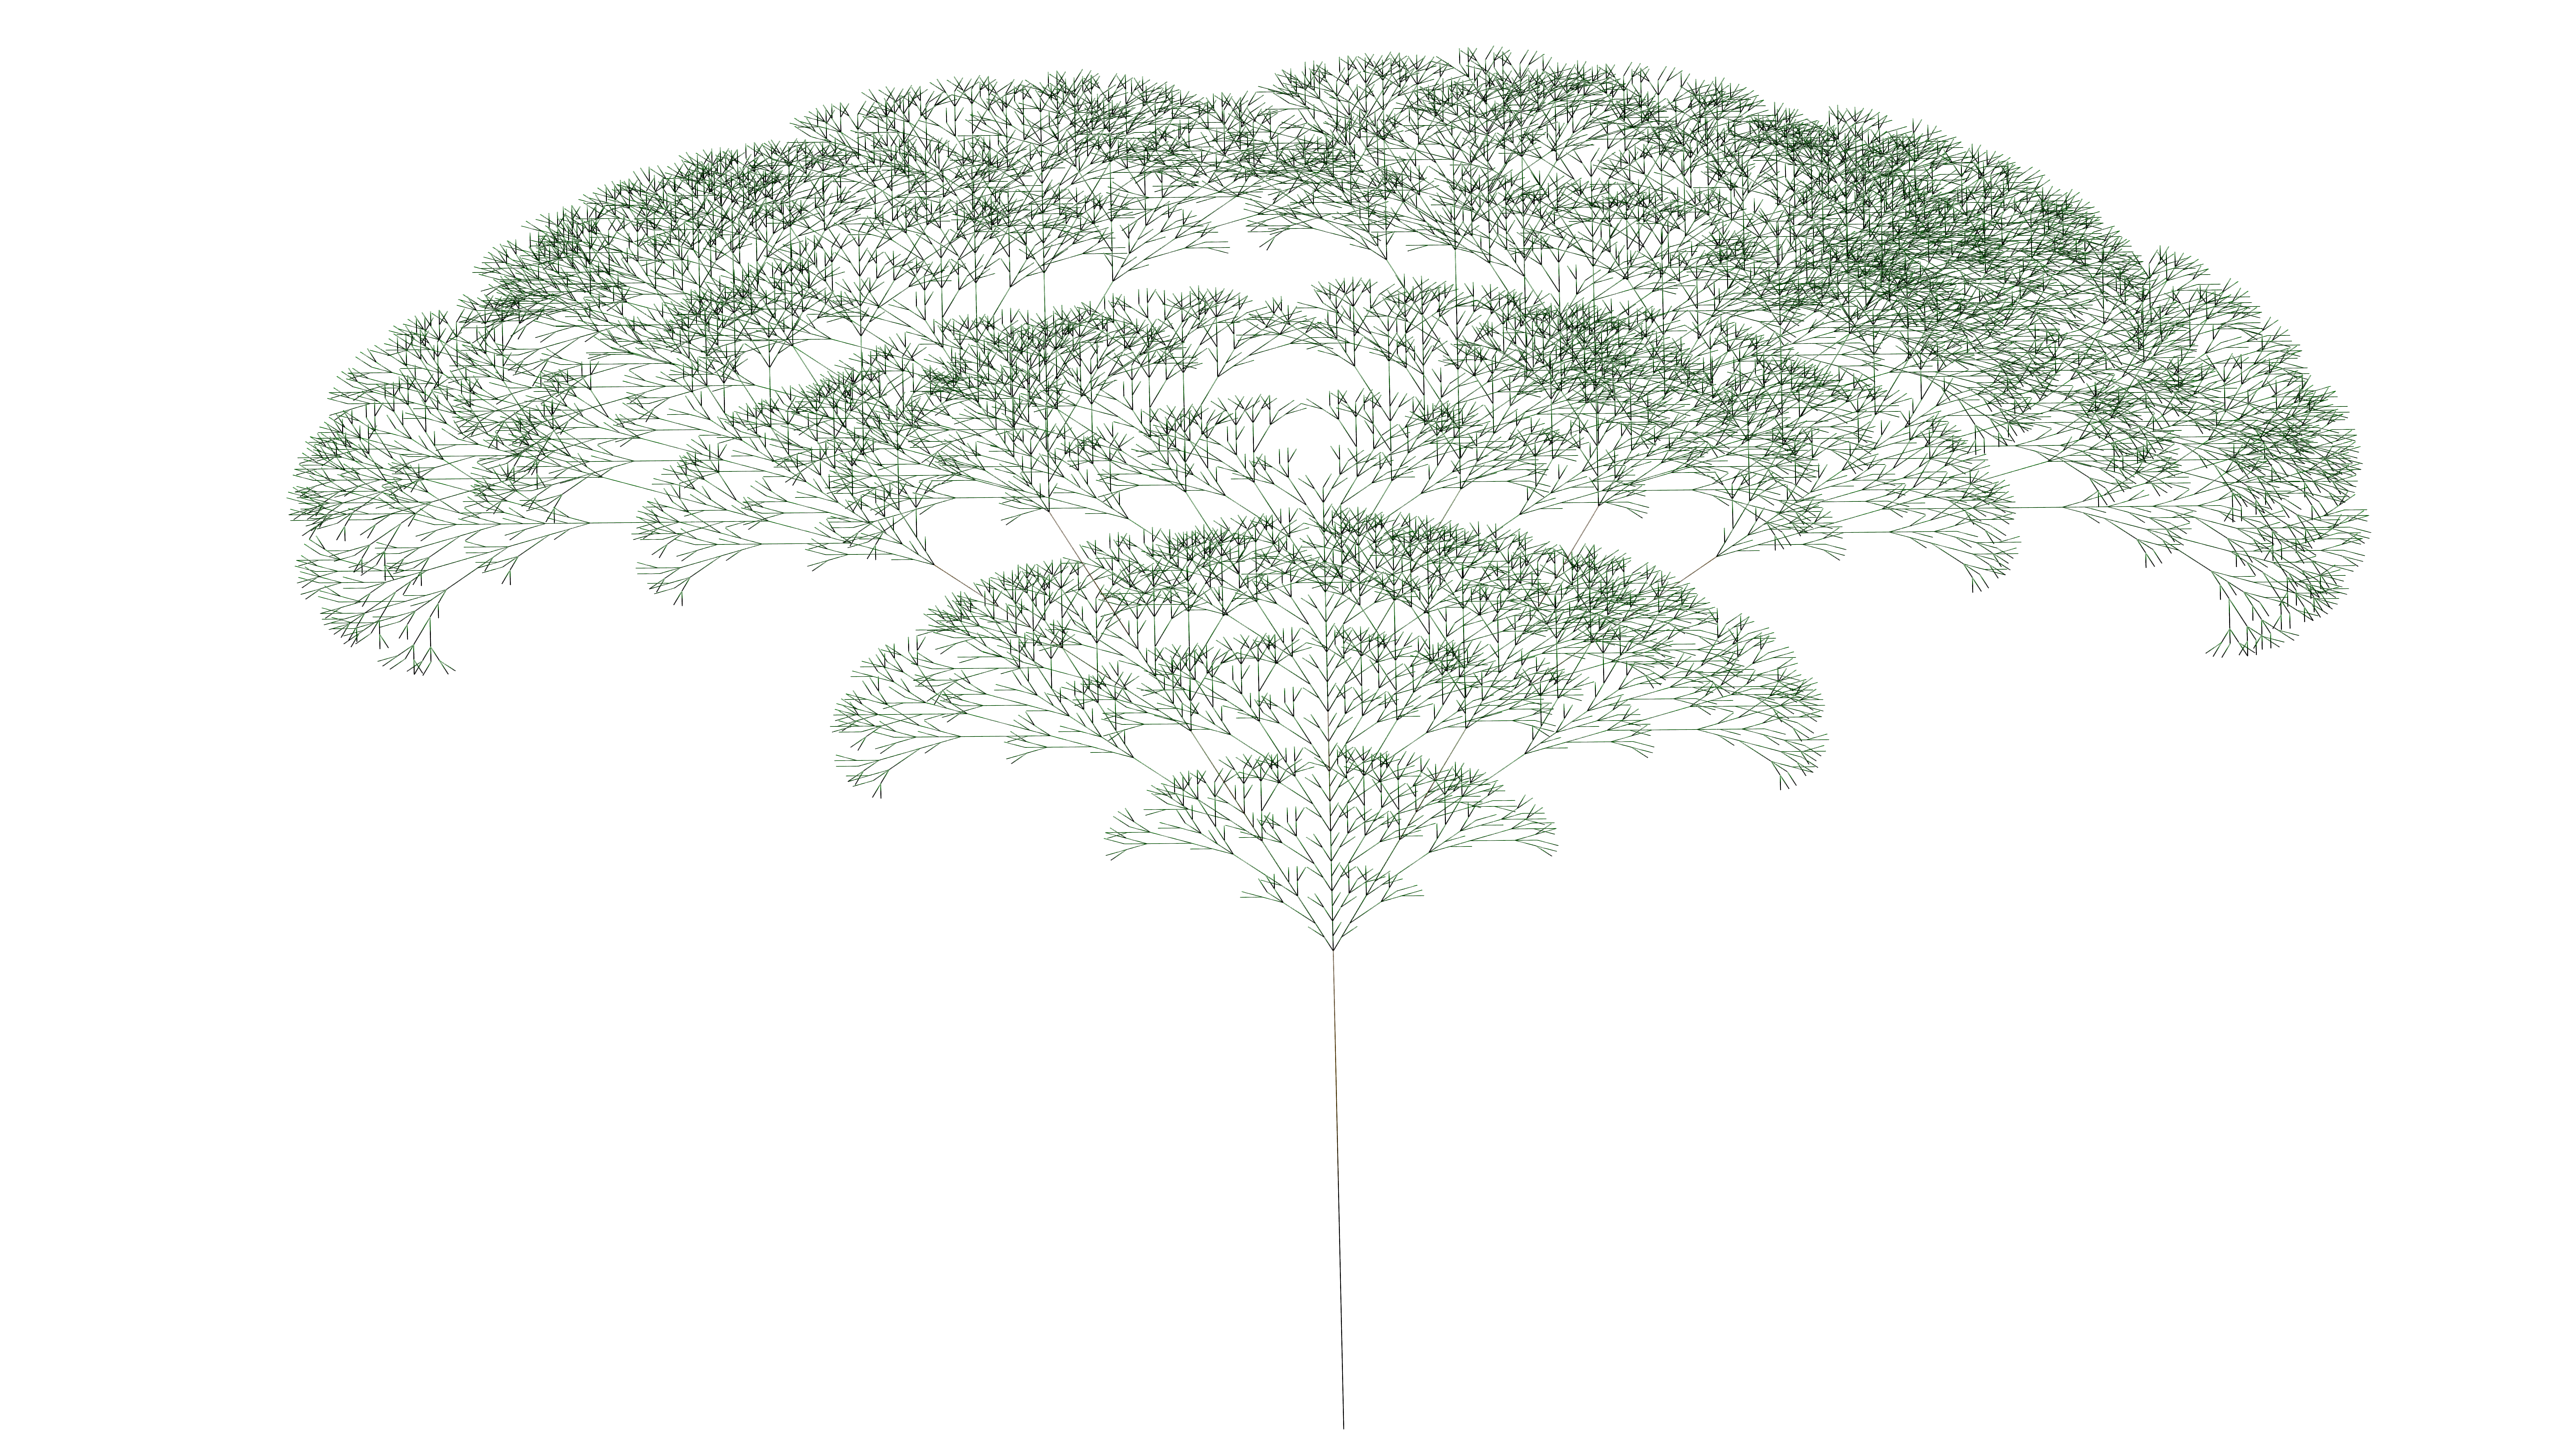
\includegraphics[width=0.90\textwidth]{figures/L-systems/f.png}
    \caption{Problem 2f}\label{fig:prob2f}
\end{figure}

\subsubsection{Expanding the Lindenmayer Systems to 3D}
We attempted to add an extra dimension to each of the items in Section
\ref{sec:p2-results}. We also experimented with classical systems such as
Sierpiński triangle, Cantor Set, Dragon, Koch, and variants of our own design.

% \todoinline[caption=3d results]{
%     Discuss how to create more interesting 3D fractals, including Koch curves, the dragon curve, and 3D trees/bushes.

%     Show the results from \texttt{data/a.json} with the book's parameters.
% }

\subsection{Conclusion}
Following the book examples were extremely simple to implement, we simply
created \texttt{JSON} files that matched the book description. To build the 3D
variants we experimented until they looked decent. The other variants were
through trial and error or online examples. It was fun to play with the
different rules and attempt to get structures that were uniform but didn't
entirely look uniform.

% !TeX root = ../hw4.tex
\section{Generating a Fractal Landscape}

\subsection{Statement}
Implement the random midpoint displacement algorithm in two dimensions to generate some fractal landscapes.
Examine the influence of $H$ on the generated landscapes.

\subsection{Method}
\autoref{prob3:alg:rmd1d} gives the random midpoint displacement algorithm for generating a random 1-dimensional vector.
Note that the dimensions of this vector are determined by the number of recursive subdivisions of the domain.

\begin{algorithm}[H]
    % \begin{noindent}
    \begin{algorithmic}
        \Function{RandomMidpoint1D}{$nrc$, $\sigma$, $seed$}
            \State{Seed the RNG with $seed$}
            \State{$N \gets 2^{nrc}$}\IComment{$N+1$ is the length of the generated vector}
            \State{$x_0 \gets 0$}\IComment{Initialize the height of both ends of the vector}
            \State{$x_N \gets \sigma \cdot \mathrm{randn()}$}
            \For{$i \in \{1, \dots, nrc\}$}
                \State{$\vec \Delta_i \gets \sigma \cdot 0.5^{(i + 1) / 2}$}\IComment{Compute the variances for each point}
            \EndFor{}
            \State\Call{Recurse}{$\vec x$, $0$, $N$, $1$, $nrc$}
            \State\Return{$\vec x$}
        \EndFunction{}
        \Function{Recurse}{$\vec x$, $t_0$, $t_2$, $t$, $nrc$}
            \State{$t_1 \gets (t_0 + t_2) / 2$}
            \State{$x_{t_1} \gets \frac{1}{2}\cdot(x_{t_0} + x_{t_2}) + \Delta_t \cdot \mathrm{randn()}$}
            \If{$t < nrc$}\IComment{Recursively fill the rest of the vector $\vec x$}
                \State\Call{Recurse}{$\vec x$, $t_0$, $t_1$, $t+1$, $nrc$}
                \State\Call{Recurse}{$\vec x$, $t_1$, $t_2$, $t+1$, $nrc$}
            \EndIf{}
        \EndFunction{}
    \end{algorithmic}
    % \end{noindent}
    \caption{The random midpoint displacement algorithm in one dimension}\label{prob3:alg:rmd1d}
\end{algorithm}

This algorithm effectively generates a random heightmap above a regularly spaced segment of the real number line.
The extension of the algorithm to two dimensions would generate a heighmap above a square 2D grid --- effectively generating a landscape heightmap.

To do so, we must modify \autoref{prob3:alg:rmd1d} to generate a square matrix of random values, and recursively quadsect this matrix until we have reached the recursion limit $nrc$.
This is shown in \autoref{prob3:alg:rmd2d}.

\begin{algorithm}[H]
    % \begin{noindent}
    \begin{algorithmic}
        \Function{RandomMidpoint2D}{$nrc$, $\sigma$, $seed$}
            \State{Seed the RNG with $seed$}
            \State{$N \gets 2^{nrc}$}\IComment{$N+1$ is the length of one side of the square matrix}
            \State{$X_{0,0}, X_{0,N}, X_{N,0}, X_{N,N} \gets \sigma \cdot \mathrm{randn()}$}\IComment{Initialize each of the matrix corners}
            \For{$i \in \{1, \dots, nrc\}$}
                \State{$\Delta_i \gets \sigma \cdot \frac{1}{2}^{(i + 1) / 2}$}
            \EndFor{}
            \State\Call{Recurse2D}{$X$, $(0, 0)$, $(N, 0)$, $(N, N)$, $(0, N)$, $1$, $nrc$}\IComment{Corners in CW order}
        \EndFunction{}
        \Function{Recurse2D}{$X$, $(x_0, y_0)$, $(x_2, y_0)$, $(x_2, y_2)$, $(x_0, y_2)$, $t$, $nrc$}
            \State{$x_1 \gets (x_0 + x_2) / 2$}
            \State{$y_1 \gets (y_0 + y_2) / 2$}
            \State{$X_{x_0, y_1} \gets \frac{1}{2}\big(X_{x_0, y_0} + X_{x_0, y_2}\big) + \Delta_t \cdot \mathrm{randn()}$}
            \State{$X_{x_1, y_0} \gets \frac{1}{2}\big(X_{x_0, y_0} + X_{x_2, y_0}\big) + \Delta_t \cdot \mathrm{randn()}$}
            \State{$X_{x_2, y_1} \gets \frac{1}{2}\big(X_{x_2, y_0} + X_{x_2, y_2}\big) + \Delta_t \cdot \mathrm{randn()}$}
            \State{$X_{x_1, y_2} \gets \frac{1}{2}\big(X_{x_0, y_2} + X_{x_2, y_2}\big) + \Delta_t \cdot \mathrm{randn()}$}
            \State{$X_{x_1, y_1} \gets \frac{1}{4}\big(X_{x_0, y_1} + X_{x_1, y_0} + X_{x_2, y_1} + X_{x_1, y_2}\big) + \Delta_t \cdot \mathrm{randn()}$}
            \If{ $t < nrc$}
                \State\Call{Recurse2D}{$X$, $(x_0, y_0)$, $(x_1, y_0)$, $(x_1, y_1)$, $(x_0, y_1)$, $t+1$, $nrc$}
                \State\Call{Recurse2D}{$X$, $(x_1, y_0)$, $(x_2, y_0)$, $(x_2, y_1)$, $(x_1, y_1)$, $t+1$, $nrc$}
                \State\Call{Recurse2D}{$X$, $(x_1, y_1)$, $(x_2, y_1)$, $(x_2, y_2)$, $(x_1, y_2)$, $t+1$, $nrc$}
                \State\Call{Recurse2D}{$X$, $(x_0, y_1)$, $(x_1, y_1)$, $(x_1, y_2)$, $(x_0, y_2)$, $t+1$, $nrc$}
            \EndIf{}
        \EndFunction{}
    \end{algorithmic}
    % \end{noindent}
    \caption{The 2D extension of \autoref{prob3:alg:rmd1d}}\label{prob3:alg:rmd2d}
\end{algorithm}

Modifying both algorithms to work with fractional Brownian motion involves changing the $\Delta_t$ update step for each recursive level from
\begin{equation}
    \Delta_t = \sigma \cdot \frac{1}{2}^{(t + 1) / 2}\label{prob3:eqn:rmd-Delta}
\end{equation}
to
\begin{equation}
    \Delta_t = \sqrt{\frac{\sigma^2}{2^{2tH}} \big(1 - 2 ^ {2 H - 2}\big)}\label{prob3:eqn:fBm-Delta}
\end{equation}

Then the parameter $H$, called the Hurst exponent, describes the roughness of the fractal.
The book indicates lower values of $H$ should \textit{increase} the fractal roughness, while higher values will decrease the roughness.

Also note that the fractal's dimension can be recovered from $H$
\begin{equation}
    d = 2 - H\label{prob3:eqn:fractal-dimension-1d}
\end{equation}
for the 1D random midpoint algorithm, and
\begin{equation}
    d = 3 - H\label{prob3:eqn:fractal-dimension-2d}
\end{equation}
for the 2D version.
Thus smaller $H$ values \textit{increase} the fractal dimension, while larger values decrease the fractal dimension.

\subsection{Implementation}
\subsection{Results}
\subsection{Conclusion}


\part{Cellular Automata}
\begin{figure}[H]
    \centering
    \includegraphics[width=\textwidth]{figures/reactions/kappa.eps}
\end{figure}
% !TeX root = ../hw4.tex
\section{Heatflow Simulation}

\subsection{Statement}
Implement a CA simulation of 2D heat flow.
Assume the domain is $0 < x < 10$, $0 < y < 10$, with insulated boundary conditions on the top and bottom.
Also assume that the right side is held at a constant zero degrees and the left side has a constant temperature profile of $y(10 - y)$.
Use a $100 \times 100$ grid.

Generate several plots of the temperature profile at fixed values of time.

\subsection{Method}
We used a classic cellular automata system, with rules
\begin{align*}
    U_{i, j} & = \frac{1}{4}\big( U_{i + 1, j} + U_{i - 1, j} + U_{i, j + 1} + U_{i, j - 1} \big) & \text{(4-neighbor average)} \\
    U_{0, j} & = U_{1, j}                                                                         & \text{(top no-flux)}        \\
    U_{n, j} & = U_{n - 1, j}                                                                     & \text{(bottom no-flux)}     \\
\end{align*}
because diffusion without advection can be modeled by a simple 4-neighbor average.
The no-flux boundary conditions on the top and bottom boundaries are handled by updating only the interior cells per iteration, and then updating the top and bottom rows of cells at the end of the iteration according to the rules above.
The constant temperature profiles on the left and right boundaries are handled by the CA initialization only, because we will not iterate over the boundary cells.

\subsection{Implementation}
A single time step for the CA can be implemented as
\begin{minted}{python}
    @numba.njit(cache=True)
    def step(grid, temp):
        """Perform one time step of a 2D diffusion CA."""
        rows, cols = grid.shape
        # Do not update any of the four boundaries.
        for row in range(1, rows - 1):
            for col in range(1, cols - 1):
                left, right = col - 1, col + 1
                top, bottom = row - 1, row + 1
                # Perform a four neighbor average.
                temp[row, col] = (
                    grid[top, right] + grid[top, left] + grid[bottom, right] + grid[bottom, left]
                ) / 4
        # Update the values of the top and bottom rows to have no flux boundary conditions.
        temp[0, :] = temp[1, :]
        temp[-1, :] = temp[-2, :]
        grid[:, :] = temp[:, :]
\end{minted}
Notice that the loop variables \mintinline{python}{row} and \mintinline{python}{col} do not loop over the four boundaries of the grid.

The grid initialization and repeated timestepping can be implemented as
\begin{minted}{python}
    def istep(rows, cols, ymin, ymax):
        domain = np.zeros((rows, cols))
        domain[:, 0] = np.linspace(ymin, ymax, cols) * (10 - np.linspace(ymin, ymax, rows))
        temporary = domain.copy()
        while True:
            step(domain, temporary)
            yield domain
\end{minted}
Notice that this is implemented as an infinite iterator.
This allows for the caller to compose this iterator with their own consumer iterator that could possibly modify the values in the grid to simulate more complicated behavior.\footnote{This behavior has been observed by the dynamical systems gremlins that haunt the McLaury building.}

\subsection{Results}
Our results were as expected.
\autoref{prob4:fig:diffusion-simple} shows the domain after 2000 timesteps.\footnote{I don't know where the weird grid patterns are coming from. They are not present in the generated EPS image --- the only show up after the \LaTeX{} document has been compiled\dots}

\begin{figure}[H]
    \centering
    \includegraphics[width=0.6\textwidth]{figures/heat/diffusion-simple.eps}
    \caption{The domain after 2000 timesteps}\label{prob4:fig:diffusion-simple}
\end{figure}

\autoref{prob4:fig:diffusion-time} shows the domain at 9 different time slices spaced 200 timesteps apart.
\begin{figure}[H]
    \centering
    \includegraphics[width=0.8\textwidth]{figures/heat/diffusion-time.eps}
    \caption{The domain after 1800 timesteps}\label{prob4:fig:diffusion-time}
\end{figure}

% !TeX root = ../hw4.tex
\section{Reproducing the Gray-Scott Model Results}

\subsection{Statement}
Reproduce the Gray-Scott patterns $\alpha$, $\lambda$, $\mu$, and $\theta$ shown in \autoref{prob5:fig:patterns}.

\begin{figure}[H]
    \centering
    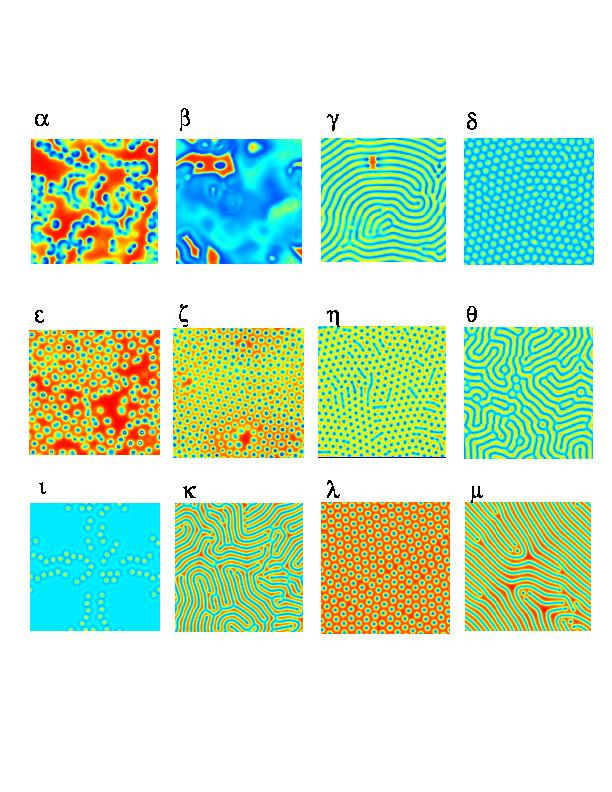
\includegraphics[width=0.6\textwidth]{figures/reactions/patterns.jpg}
    \caption{The labeled Gray-Scott patterns}\label{prob5:fig:patterns}
\end{figure}

\subsection{Method}

The Gray-Scott Model models reaction diffusion of two chemicals $U$ and $V$ in an unstirred planar chemical reactor.
Further, we assume the reaction $U \to V$ is autocatalyzed by the presence of $V$.
More specifically, the Gray-Scott model assumes the cubic autocatalysis
\begin{equation}
    U + 2V \to 3V
\end{equation}
with reaction rate $kuv^2$.
This reaction can be modeled according to the following system of differential equations.\footnote{I'm smashing my giant red ``I Believe'' button on this one. My chemistry is a little rusty, and PDEs give me heart palpitations.}
\begin{equation}
    \begin{cases}
        \displaystyle{\frac{\partial u}{\partial t} = r_u \Delta u - uv^2 + f(1 - u)} \\[10pt]
        \displaystyle{\frac{\partial v}{\partial t} = r_v \Delta v + uv^2 - (f + k)v}
    \end{cases}\label{prob5:eqn:gray-scott}
\end{equation}
where $u$ and $v$ are the concentrations, and $r_u$ and $r_v$ are the diffusion rates, of $U$ and $V$ respectively.
The chemical $U$ is added to the reactor at the feed rate $f$ which is scaled by the concentration of $U$.
Simultaneously, $U$ and $V$ are drained from the reactor at the kill rate $k$, which is scaled by $f$ and the concentration of $V$.

Recall that the Laplacian operator $\displaystyle\Delta f(x, y, t) = \nabla^2 f(x, y, t) = \frac{\partial^2 f}{\partial x^2} + \frac{\partial^2 f}{\partial y^2}$ can be discretized as
\begin{align}
    \Delta f(x, y, t) \approx \frac{f(x - h, y, t) + f(x + h, y, t) + f(x, y - h, t) + f(x, y + h, t) - 4f(x, y)}{h^2}\label{prob5:eqn:discrete-laplacian-operator}
\end{align}
for fixed step size $h$, uniform in both spatial dimensions --- allowing us to collect more of the terms together.
In this problem, we have $\Delta x = \Delta y = \Delta t = h = 1$.

However, note that the numerical computation of $\Delta f$ over a large spatial domain is computationally intensive, despite being relatively simple.
Therefore, we desire a a method where the Laplacian can be applied to $f$ over each element of the spatial domain at once.

Let $\mathbf U$ be a square $n \times n$ matrix of concentrations.
We then unravel $\mathbf U$ into a column vector $\vec u$ and left-multiply by an $n^2 \times n^2$ matrix $\mathbf L$ to numerically compute the discrete Laplacian over the entire spatial domain.

That is, the discretized version of \autoref{prob5:eqn:gray-scott} becomes
\begin{eqnarray}
    \begin{cases}
        \vec u_{t + 1} & = \vec u_t + r_u \mathbf L \cdot \vec u_t - \vec u_t \cdot \vec {v_t}^2 + f(1 - \vec u_t) \\
        \vec v_{t + 1} & = \vec v_t + r_v \mathbf L \cdot \vec v_t + \vec u_t \cdot \vec {v_t}^2 - (f + k)\vec v_t
    \end{cases}\label{prob5:eqn:discretized-gray-scott}
\end{eqnarray}
where the vector product $\vec u_t \cdot \vec {v_t}^2$ is computed component-wise.

Then the $n ^2 \times n^2$ matrix $\mathbf L$ is the block diagonal matrix
\begin{equation}
    \mathbf L = \begin{bmatrix}
        L_n    & I_n    & 0_n    & \cdots & 0_n    & I_n    \\
        I_n    & L_n    & I_n    & 0_n    & \cdots & 0_n    \\
        0_n    & I_n    & L_n    & I_n    & \ddots & \vdots \\
        \vdots & \ddots & \ddots & \ddots & \ddots & 0_n    \\
        0_n    & \cdots & 0_n    & I_n    & L_n    & I_n    \\
        I_n    & 0_n    & \cdots & 0_n    & I_n    & L_n
    \end{bmatrix}\label{prob5:eqn:laplacian}
\end{equation}
where the $0_n$ blocks are the $n \times n$ zero matrix, and the $I_n$ blocks are the $n \times n$ identity matrix.
The $L_n$ blocks are the $n \times n$ diagonal matrix
\begin{equation}
    L_n = \begin{bmatrix}
        -4     & 1      & 0      & \cdots & 0      & 1      \\
        1      & -4     & 1      & 0      & \cdots & 0      \\
        0      & 1      & -4     & 1      & \ddots & \vdots \\
        \vdots & \ddots & \ddots & \ddots & \ddots & 0      \\
        0      & \cdots & 0      & 1      & -4     & 1      \\
        1      & 0      & \cdots & 0      & 1      & -4
    \end{bmatrix}\label{prob5:eqn:laplacian-L-block}
\end{equation}

Now, $\mathbf L$ is appropriate for periodic boundary conditions.
If homogeneous Dirichlet boundary conditions are desired, we use the matrix
\begin{equation}
    \mathbf L_d = \begin{bmatrix}
        L_n              & I_n    & 0_n    & \cdots & 0_n    & \color{red}{0_n} \\
        I_n              & L_n    & I_n    & 0_n    & \cdots & 0_n              \\
        0_n              & I_n    & L_n    & I_n    & \ddots & \vdots           \\
        \vdots           & \ddots & \ddots & \ddots & \ddots & 0_n              \\
        0_n              & \cdots & 0_n    & I_n    & L_n    & I_n              \\
        \color{red}{0_n} & 0_n    & \cdots & 0_n    & I_n    & L_n
    \end{bmatrix}
\end{equation}
and the modified $L_n$ block
\begin{equation}
    L_n = \begin{bmatrix}
        -4             & 1      & 0      & \cdots & 0      & \color{red}{0} \\
        1              & -4     & 1      & 0      & \cdots & 0              \\
        0              & 1      & -4     & 1      & \ddots & \vdots         \\
        \vdots         & \ddots & \ddots & \ddots & \ddots & 0              \\
        0              & \cdots & 0      & 1      & -4     & 1              \\
        \color{red}{0} & 0      & \cdots & 0      & 1      & -4
    \end{bmatrix}
\end{equation}
If homogeneous Neumann boundary conditions are desired, further modifications must be made to the main diagonal of $\mathbf L_d$ to maintain 0-sum rows.\footnote{
    Online material on the discretized Laplacian is lacking in general, and much more so related to periodic boundary conditions.
    I found exactly one source that discussed the discretized Laplacian with periodic boundary conditions in more than one sentence.

    A PDF of \textit{Computational Methods for Inverse Problems} may be found on \href{http://booksdescr.org/item/index.php?md5=6DF2AA596DDBE34BCF9354A5626B75DA}{Library Genesis}.
    The relevant pages are 74--75.
}

\subsection{Implementation}
\subsection{Results}
The $f$ and $k$ parameters largely decide the pattern displayed at the end of a large number of iterations.
The mappings for the patterns shown in \autoref{prob5:fig:patterns} are shown in \autoref{prob5:fig:pattern-mappings}.
\begin{figure}[H]
    \centering
    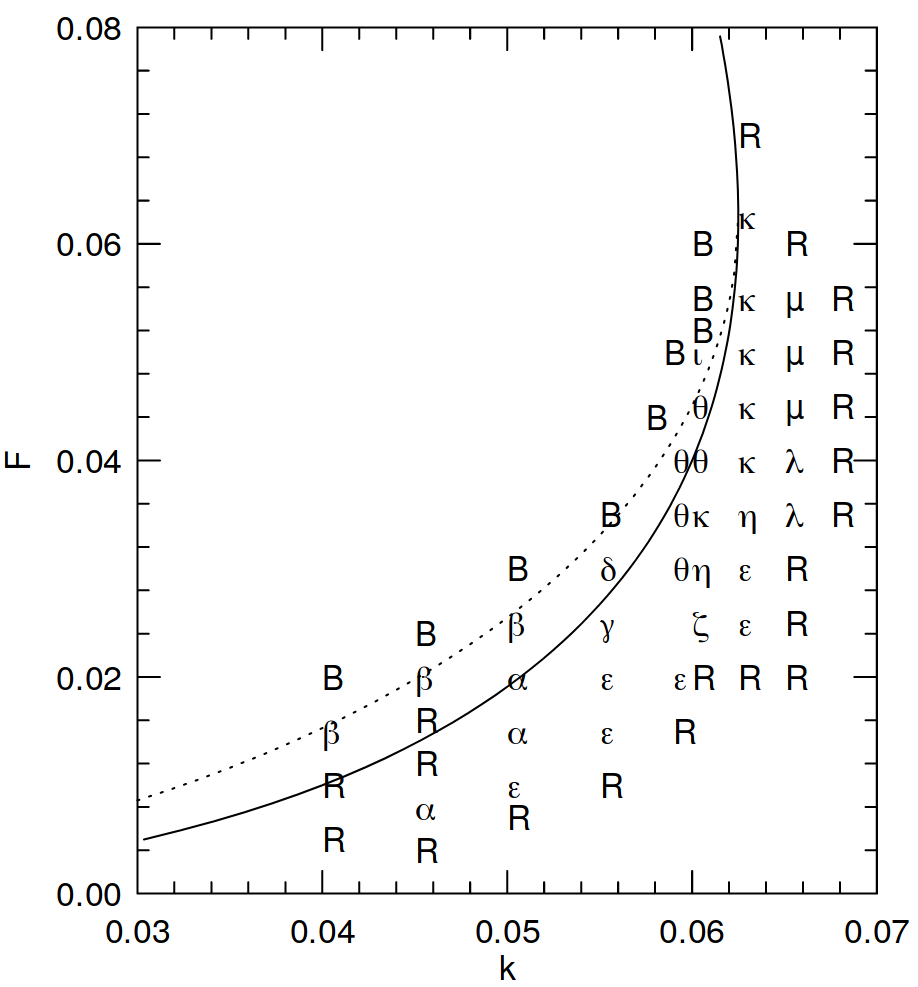
\includegraphics[width=0.6\textwidth]{figures/reactions/pattern-mappings.png}
    \caption{The parameter mappings to the patterns shown in \autoref{prob5:fig:patterns}}\label{prob5:fig:pattern-mappings}
\end{figure}
\subsection{Conclusion}


\end{document}
